\documentclass{iutbscthesis}
\usepackage{kantlipsum} % This package is used to generate place holder text. Remove it in the actual world.

\tolerance=1 % Allow some flexibility for line breaking
\emergencystretch=\maxdimen % Allow line breaking to stretch a little more
\hyphenpenalty=10000 % Allow hyphenation with a reasonable penalty
\hbadness=10000 % Suppress most warnings about underfull or overfull lines

% The iutbscthesis uses biblatex for bibliography management.
% You can learn the basics of biblatex from:
% https://www.overleaf.com/learn/latex/Bibliography_management_with_biblatex
\addbibresource{citations.bib}
\graphicspath{{./figures/}}
\DeclareGraphicsExtensions{.pdf, .png, .jpg, .jpeg}


% The complete title of your thesis, mandatory
\title{\Large{Weakly Supervised Semantic Segmentation with better CAMs using UniCL and Swin Transformers}}

% Use the \addauthor command to keep adding authors with student ID
\addauthor{Anika Farzana}{200041204}
\addauthor{K. M. Abesh Ahsan}{200041225}
\addauthor{Sayema Amin}{200041234}

% Use the \supervisor command to define the supervisor with name, designation, and department
% There needs to be one and only one supervisor
\supervisor{Dr. Hasanul Kabir}{Professor}{Department of Computer Science and Engineering}

% Use the \addcosupervisor command to add a cosupervisor. There might be no cosupervisor at all
% % In that case, just remove all of the \addcosupervisor commands.
% \addcosupervisor{Dr.\ Sue Permann}{Assistant Professor}{Department of Computer Science and Engineering}
% \addcosupervisor{Mr. Francis FullOfFrenchPeople}{Lecturer}{Department of Computer Science and Engineering}

% Complete department name, mandatory
\department{Department of Computer Science and Engineering}

% Complete program name, mandatory
\program{BACHELOR OF SCIENCE IN COMPUTER SCIENCE AND ENGINEERING}

% Date (day, month name, and year) when the presentation took place, mandatory
\defensedate{29}{April}{2025}

\begin{document}

%-------------------------- FRONT MATTER --------------------------%

% Generate cover page of the report to be printed on the hard cover
\coverpage

% Switch to roman page numbering
\pagenumbering{roman}

% Generate the title leaf, mandatory
\titlepage

% Auto generate declaration of candidate based on previous info, mandatory
\declarationofcandidate

% % Dedicate report to someone. You may add more sentences to it.
% \dedicatedto{our supervisor without whom this degree would have been completed six months earlier}

\tableofcontents
\listoffigures
\listoftables

\clearpage

% Add abbreviations within this environment using the \abbr command
% \begin{abbreviations}
%     \abbr{CNN}{Convolutional Neural Network}
%     \abbr{PIP}{PIP Installs Packages}
%     \abbr{TikZ}{TikZ ist kein Zeichenprogramm}
%     \abbr{WIKI}{What I Know Is}
% \end{abbreviations}

% Any acknowledgement that you want to write goes in the following environment

\begin{acknowledgement}
    I am profoundly grateful to my supervisor, Dr. Hasanul Kabir, Professor, Department of Computer Science and Engineering, for his outstanding guidance, support, and feedback throughout this research journey. His expertise and encouragement have been pivotal in shaping the direction and quality of this thesis.

His patience and dedication to his work have inspired me to aim for excellence and approach challenges with curiosity and determination. His constructive feedback and insightful suggestions have significantly deepened my understanding of the domain and inspired me to think critically and creatively.

It has been an honor to work under his supervision, and I deeply appreciate his invaluable time and effort in guiding me through this research.
\end{acknowledgement}

% Write your abstract here.
\begin{abstract}
Semantic segmentation is a key task in computer vision that involves interpreting images at the pixel level. While fully supervised methods provide high accuracy, they require extensive pixel-level annotations, making them resource-intensive. Weakly Supervised Semantic Segmentation (WSSS) addresses this issue by using weaker supervision formats like image-level labels, reducing the need for annotation while still training effective segmentation models.

Recent WSSS advancements have shown that competitive performance can be reached with minimal labeled data through the use of Class Activation Maps (CAMs). However, challenges such as sparsity and inadequate boundary delineation affect CAM quality.

This study aims to improve CAM quality by exploring effective backbone architectures and refinement strategies. We investigate multi-modal architectures like UniCL and hierarchical transformers such as Swin Transformer to enhance feature extraction. To further refine CAMs, we use an affinity-based framework that combines decoder-derived affinities with attention maps, creating more semantically coherent pseudo-labels. Additionally, we incorporate a Pixel-Adaptive Refinement (PAR) module to refine pseudo-labels based on local similarities, ensuring better object boundaries.

Our experiments demonstrate that UniCL and Swin Transformer can localize objects more effectively and precisely, thus generating better CAMs than than traditional transformers. 
\end{abstract}

%-------------------------- MAIN BODY --------------------------%
% Switch to arabic page numbering
\pagenumbering{arabic}

% \chapter{Introduction}
\label{chap:introduction}

\section{Semantic Segmentation}
\label{sec:semantic_segmentation}
Semantic segmentation is a fundamental task in computer vision that involves partitioning an image into semantically meaningful regions. Each pixel in the image is assigned a label corresponding to the object or region it belongs to. This task is crucial for applications such as autonomous driving, medical image analysis, and scene understanding.

The goal of semantic segmentation is to achieve pixel-level understanding of an image, which is more detailed than traditional image classification or object detection. Unlike these tasks, semantic segmentation requires not only identifying the presence of objects but also delineating their precise boundaries.


\subsection{Fully Supervised Semantic Segmentation}
\label{subsec:fully_supervised}
Fully supervised semantic segmentation methods rely on large amounts of labeled data, where each pixel in the training images is annotated with its corresponding class label. These methods typically use deep learning architectures, such as convolutional neural networks (CNNs), to learn complex features and patterns from the labeled data. The performance of these models is heavily dependent on the quality and quantity of the annotated data.

\subsection{Weakly Supervised Semantic Segmentation}
\label{subsec:weakly_supervised}
Weakly supervised semantic segmentation aims to reduce the reliance on extensive pixel-level annotations by utilizing weaker forms of supervision, such as image-level labels, bounding boxes, or scribbles. This approach allows for the training of segmentation models with limited labeled data while leveraging large amounts of unlabeled data. Weakly supervised methods have gained popularity due to their ability to achieve competitive performance with significantly less annotation effort.

\section{Motivation}
\label{sec:motivation}

Semantic segmentation has established itself as a fundamental task in computer vision, with broad applications in areas such as autonomous driving, medical imaging, and robotics. In these domains, a precise pixel-level understanding of the environment is not merely desirable but often critical: for example, safe navigation of self-driving vehicles relies on reliable scene parsing, and accurate delineation of anatomical structures can directly impact medical diagnosis and treatment.

Despite its importance, conventional semantic segmentation has been heavily reliant on fully supervised learning. This paradigm demands large-scale datasets with dense pixel-level annotations, which are costly and labor-intensive to produce. Annotating high-resolution images can take hours per image, and the process remains prone to human error. Beyond annotation effort, fully supervised methods face additional hurdles: (i) class imbalance in real-world datasets often biases models toward dominant categories, (ii) complex scenes with occlusion, lighting variation, and fine structural detail challenge the robustness of predictions, and (iii) models trained on specific datasets frequently fail to generalize across domains due to dataset-specific biases.

These challenges naturally motivate the exploration of weakly supervised semantic segmentation (WSSS). By replacing dense annotations with weaker forms of supervision—such as image-level labels, bounding boxes, or scribbles—WSSS reduces annotation cost while still enabling model training. The key idea is to leverage weak supervision to generate class activation maps (CAMs) and corresponding pseudo-labels, which can then guide the segmentation process. Although CAMs are often coarse or noisy, refinement strategies allow them to approximate dense ground truth, making WSSS a practical compromise between annotation effort and segmentation performance.

The motivation for this research is thus twofold: first, to address the scalability and practicality issues of fully supervised methods, and second, to improve the quality and reliability of WSSS pipelines. By advancing WSSS, we aim to narrow the performance gap with fully supervised segmentation while ensuring that solutions remain feasible for deployment in diverse and data-constrained real-world scenarios.



\section{Problem Statement}
\label{sec:problem_statement}

Weakly Supervised Semantic Segmentation (WSSS) presents a compelling alternative to fully supervised methods by significantly reducing the dependence on costly pixel-level annotations. However, current WSSS techniques rely on Class Activation Maps (CAMs) \cite{cam} generated from image-level labels to identify object regions. While this approach has shown promise, it often falls short in terms of spatial precision and completeness, leading to suboptimal segmentation results.

In the context of WSSS, the challenge lies in effectively leveraging the image-level labels to produce accurate and detailed segmentation maps. The dependence on CAMs, which are typically generated from global features, can result in sparse and coarse activation maps that fail to capture the fine details of object boundaries. This limitation is particularly pronounced when dealing with complex scenes or occlusions, where precise localization is crucial.

Additionally, the refinement techniques applied to these CAMs often fail to fully leverage the rich affinity information inherent in modern transformer architectures. Consequently, the resulting pseudo-labels lack the spatial precision required for high-quality segmentation, ultimately impacting the overall performance. This highlights the need for more robust backbone architectures capable of effectively capturing both local and global features, as well as advanced CAM refinement strategies to narrow the performance gap between weakly and fully supervised segmentation methods.

So, keeping in mind the above challenges, we aim to develop a weakly supervised semantic segmentation model that can effectively leverage image-level labels to produce accurate and detailed segmentation maps. Our approach will focus on enhancing the spatial precision and completeness of the generated CAMs.

\section{Challenges of Semantic Segmentation}
\label{sec:challenges_of_semantic_segmentation}
Semantic segmentation faces several challenges that hinder its widespread adoption and effectiveness:

\section{Challenges of Weakly Supervised Semantic Segmentation}
\label{sec:challenges_of_wsss}

While weakly supervised semantic segmentation (WSSS) reduces the annotation burden compared to fully supervised methods, it introduces its own set of challenges:

\begin{itemize}
    \item \textbf{Incomplete Object Localization:} Class activation maps (CAMs) derived from image-level labels typically highlight only the most discriminative regions, leaving large portions of the object unlabeled.
    \item \textbf{Noisy Pseudo-labels:} The process of refining CAMs into pixel-level labels often introduces noise and errors, which can propagate during training and degrade performance.
    \item \textbf{Boundary Precision:} Weak supervision lacks explicit boundary cues, making it difficult to segment fine object details and separate adjacent instances accurately.
    \item \textbf{Background Confusion:} Without strong pixel-level supervision, models often misclassify diverse background regions as foreground, or vice versa.
    \item \textbf{Multi-class Co-occurrence:} In scenes containing multiple objects, weak labels struggle to capture clear distinctions, leading to overlapping or missing class activations.
    \item \textbf{Class Imbalance:} Underrepresented classes may not produce strong activations in CAMs, resulting in poor segmentation for rare categories.
    \item \textbf{Dependence on External Cues:} Many WSSS methods rely on saliency maps or additional priors to improve CAMs, but these external cues may be dataset-specific and limit generalization.
\end{itemize}

Addressing these challenges is crucial for advancing WSSS methods toward practical applications where annotation resources are limited.


\section{Contribution}
\label{sec:contribution}

In this work, we make the following key contributions:

\begin{itemize}
    \item We explore the use of the UniCL framework \cite{vl_unicl} with a Swin Transformer backbone \cite{transformer_swin} to enhance CAM generation, leveraging Swin's ability to capture both local fine details and global context through its hierarchical structure.
    \item We adapt the affinity-based CAM refinement technique from WeCLIP \cite{wsss_frozen_clip} to the Swin Transformer backbone by computing pixel affinities from Swin's hierarchical features, allowing the refinement to propagate class activations effectively despite the absence of a global attention map.
    \item We integrate a Pixel-Adaptive Refinement Module (PAR) \cite{wsss_afa_affinity_from_attention} that incorporates both color and spatial information, further refining the pseudo-labels and enhancing boundary accuracy.
    \item We integrate the refined CAMs and Pixel-Adaptive Refinement into the standard WSSS training pipeline, training the model to leverage these improved pseudo-labels for better segmentation performance.

\end{itemize}

\section{Organization}
\label{sec:organization}

The remainder of this thesis report is organized as follows:

\begin{itemize}
    \item \textbf{Chapter \ref{chap:related-works}: Related Works} provides a comprehensive review of existing literature on semantic segmentation. It discusses fully supervised and weakly supervised methods, key architectures like U-Net, DeepLab, and Vision Transformers, and identifies gaps in current research.

    \item \textbf{Chapter \ref{chap:methodology}: Proposed Methodology} details the proposed approach, including the use of the UniCL framework with a Swin Transformer backbone for CAM generation. It also describes the affinity-based CAM refinement technique and the Pixel-Adaptive Refinement Module (PAR) for pseudo-label generation and segmentation refinement.

    \item \textbf{Chapter \ref{chap:citations}: Citations} provides guidance on managing references using \texttt{biblatex}, with examples of citing articles, books, and multi-citations.

    \item \textbf{Appendices} include supplementary materials such as additional figures, tables, and extended discussions that support the main content of the thesis.
\end{itemize}

This structure ensures a logical flow, starting from the foundational concepts and related works, progressing through the proposed methodology, and concluding with the results, discussions, and supplementary materials.


% \chapter {Related Works}
\label{chap:related-works}

\section{Fully Supervised Semantic Segmentation}
\label{sec:fully-supervised}

In fully supervised semantic segmentation, the model is trained on a dataset with pixel-level annotations. The model learns to predict the class of each pixel in an image based on the provided annotations. This approach typically requires a large amount of labeled data, which can be expensive and time-consuming to obtain.

\subsection{Early Approaches}
\label{subsec:early-approaches}
The early approaches to semantic segmentation relied heavily on hand-crafted features and traditional machine learning techniques. These methods often involved extracting low-level features such as color, texture, and shape from the images and then using classifiers like Support Vector Machines (SVMs) or Random Forests to assign labels to each pixel.

Then came the era of deep learning, where convolutional neural networks (CNNs) revolutionized the field. The introduction of fully convolutional networks (FCNs) allowed for end-to-end training of segmentation models, enabling them to learn spatial hierarchies of features directly from the data. This was a significant breakthrough, as it eliminated the need for manual feature extraction and allowed for more accurate and efficient segmentation.

\subsection{Convolutional Neural Networks (CNNs)}
\label{subsec:cnn_sem_seg}

The first fully convolutional network (FCN) for semantic segmentation was proposed by \cite{fsss_fcn}, which replaced the fully connected layers in traditional CNNs with convolutional layers. This allowed the network to produce dense predictions for each pixel in the input image. The FCN architecture was further improved by adding skip connections, which helped to preserve spatial information and improve segmentation accuracy.

Then came the introduction of U-Net \cite{fsss_unet}, a popular architecture for semantic segmentation that is widely used in medical imaging and other applications. U-Net consists of an encoder-decoder structure, where the encoder captures context information and the decoder enables precise localization. The \emph{skip connections} between the encoder and decoder blocks play a crucial role by retaining spatial information, making U-Net particularly effective for tasks with limited training data.

The field of semantic segmentation has continued to evolve, with the introduction of various architectures and techniques.

The deeplab series \cite{fsss_deeplabv1, fsss_deeplabv2, fsss_deeplabv3,fsss_deeplabv3plus} introduced atrous convolution and spatial pyramid pooling to capture multi-scale context information; \cite{fsss_deeplabv1} also used a methd called CRF (Conditional Random Field) to refine the segmentation results. But it was removed in the later versions of the model. In \cite{fsss_deeplabv2}, the atrous convolution method evolved into a more general form called atrous spatial pyramid pooling (ASPP), which allows the model to capture features at multiple scales. The ASPP module consists of parallel atrous convolutions with different rates, enabling the model to learn multi-scale context information effectively. Finally \cite{fsss_deeplabv3plus} introduced a new decoder module that refines the segmentation results by combining low-level features from the encoder with high-level features from the ASPP module. This approach improves the localization of object boundaries and enhances the overall segmentation performance.

\cite{fsss_pspnet} introduced the Pyramid Scene Parsing Network (PSPNet), which uses a pyramid pooling module to capture global context information at different scales. The pyramid pooling module aggregates features from different regions of the image, allowing the model to learn rich contextual information for better segmentation.

\cite{fsss_segnet} proposed SegNet, an encoder-decoder architecture that focuses on efficient upsampling of feature maps. SegNet uses a series of convolutional and pooling layers in the encoder to extract features, followed by a corresponding decoder that upsamples the feature maps to produce the final segmentation output. The main innovation in SegNet is the use of unpooling layers, which store the indices of the max-pooling operation during encoding, instead of the feature maps themselves. This allows for more efficient memory usage and faster inference times, making SegNet suitable for real-time applications.

\subsection{Transformers}
\label{subsec:transformers}
The introduction of transformers in computer vision has led to significant advancements in semantic segmentation. Vision Transformer (ViT) \cite{transformer_vit} and its variants have shown promising results in various tasks, including semantic segmentation. ViTs leverage self-attention mechanisms to capture long-range dependencies and global context information, making them suitable for dense prediction tasks.
The years later on, the transformer-based architectures have gained popularity in semantic segmentation. \cite{transformer_swin} proposed the Swin Transformer, which introduces a hierarchical architecture with shifted windows to capture both local and global context information. The Swin Transformer has shown state-of-the-art performance on various benchmark datasets, including ImageNet-1k \cite{dataset_imagenet} for image classification and COCO \cite{dataset_coco} for object detection and \cite{dataset_ade20k} for semantic segmentation. The Swin Transformer has been widely adopted in various applications.

Leveraging the strengths of Vision Transformer, \cite{fsss_setr} first proposed the SETR (Semantic Segmentation Transformer) architecture, which replaces the traditional CNN backbone with a transformer encoder. The SETR architecture consists of a ViT encoder that processes the input image and generates a set of feature maps, followed by a decoder that upsamples the feature maps to produce the final segmentation output. The SETR model has shown competitive performance on various benchmark datasets, demonstrating the effectiveness of transformers in semantic segmentation tasks.

\cite{fsss_segmenter} proposed the Segmenter architecture, which combines a ViT backbone with a lightweight decoder for efficient semantic segmentation. The Segmenter model uses a transformer encoder to capture global context information and a simple decoder to produce the final segmentation output. The Segmenter architecture is designed to be computationally efficient while maintaining high accuracy, making it suitable for real-time applications.

\cite{fsss_segformer} introduced SegFormer, a transformer-based architecture that combines the strengths of both CNNs and transformers for semantic segmentation. SegFormer uses a hierarchical transformer encoder to capture multi-scale features and a lightweight decoder to produce the final segmentation output. The SegFormer model has shown state-of-the-art performance on various benchmark datasets, demonstrating the effectiveness of combining CNNs and transformers in semantic segmentation tasks.

The field of semantic segmentation has seen significant advancements with the introduction of various architectures and techniques. The combination of CNNs and transformers has led to improved performance and efficiency in semantic segmentation tasks. As the field continues to evolve, we can expect further innovations and breakthroughs in this area.

\subsection{Problem with Fully Supervised Semantic Segmentation}
\label{subsec:problem-with-fully-supervised}
Fully supervised semantic segmentation has achieved remarkable success, largely driven by powerful models and richly annotated datasets. However, this success comes at a significant cost: acquiring dense pixel-level annotations is both expensive and time-consuming. Each image must be meticulously labeled, often requiring expert knowledge and hours of manual effort. This high annotation burden severely limits the scalability of fully supervised methods, especially for large or specialized datasets. To overcome this bottleneck, the research community has increasingly turned toward weakly supervised semantic segmentation (WSSS) — an approach that seeks to train effective segmentation models with minimal supervision.





\section{Weakly Supervised Semantic Segmentation}
\label{sec:weakly-supervised}
Fully supervised semantic segmentation depends on pixel-level segmentation masks annotated by humans. However, generating such dense annotations is tedious, time-intensive, and costly. Furthermore, crowd-sourced annotators must undergo special training to handle the complexity of pixel-level labeling, which restricts the scale and diversity of available datasets. Consequently, most curated datasets are limited to a small set of object categories. In contrast, unlabeled or weakly annotated images can be collected in abundance, at much lower cost and in shorter time. This has motivated research into weakly supervised semantic segmentation (WSSS) to make semantic segmentation models more scalable.


\section{Types of WSSS}
\label{sec:types-weakly-supervised}
A wide range of weak supervision have been explored, including bounding boxes, scribbles, points, image-level labels,  eye tracks, free-form squiggles, or noisy web tags. Bounding boxes provide rough object boundaries, offering useful localization cues, though they still require annotators to draw accurate boxes.  Scribble-based supervision allows annotators to roughly mark object regions without outlining exact object boundaries. Point supervision, by contrast, typically uses a single annotated pixel per object, giving coarse location information. While less costly than pixel-accurate masks, these methods still involve some level of manual annotation, making large-scale labeling expensive.


\section{Image-level Label based weak supervision}
\label{sec:image-level-label}
Image-level annotation is one of the most economical and efficient settings for weakly supervised semantic segmentation. In this context, every training image has its image class labels belonging to the objects present in the image but the locations of the objects are unknown. So, the challenge is to accurately assign image-level labels to their corresponding pixels.
 
Initial approaches attempted to train segmentation models directly from image-level labels \cite{dcnn}, but performance was unsatisfactory. Later methods introduced discriminative localization techniques such as Class Activation Maps (CAMs) \cite{cam}, which highlight class-relevant regions. These coarse cues were then refined using auxiliary information such as superpixels \cite{imagelevelpixel}, segmentation proposals \cite{imagelevelpixel}, or motion information from videos \cite{wsss_motion_cues}. Some works, such as Adversarial Erasing \cite{adversarial_erasing}, expanded object coverage progressively by iteratively searching new regions. Others, like Kolesnikov and Lampert \cite{kolesnikov2016}, trained networks to approximate the dense CRF \cite{krähenbühl} applied on CAMs for refinement.

Some approaches learn to predict affinity matrices at the pixel level [36], to refine the output of dCRF through random walk. AffinityNet \cite{wsss_affinitynet} predicts class-agnostic pixel affinities to propagate CAM activations via random walks. Similarly, Seeded Region Growing (SRG) \cite{srg} expands initial seed regions using similarity criteria, while its deep learning extension DSRG \cite{wsss_dsrg_deep_seeded_region_growing} leverages high-level semantic features to grow regions more effectively. P2P \cite{pixel_to_prototype} further narrows the supervision gap by using pixel-to-prototype contrastive learning. A common limitation, however, is that most of these CNN-based methods inherit the restricted locality of convolutional features.

Recent advances incorporate transformers into WSSS \cite{camtokens, getam}. TS-CAM \cite{camtokens} leverages the global information capturing ability of ViT by combining class-token attention with CAMs. \cite{getam} refines class-specific maps by using attention gradients. MCTformer \cite{wsss_MCTformer} expands this idea by embedding multiple class tokens to learn attention maps for different categories. AFA \cite{wsss_afa_affinity_from_attention} instead derives semantic affinities directly from attention maps to refine coarse pseudo-labels. FrozenCLIP \cite{wsss_frozen_clip} pushes this further by exploiting the frozen CLIP backbone to generate high-quality pseudo-labels, which are dynamically updated using a refinement module (RFM).


\section{Stages}
\label{sec:stages}

Weakly supervised semantic segmentation has two main solutions based on their training processes: multi-stage approaches \cite{instance_wsss,wsss_L2G,wsss_rib} and single-stage approaches \cite{wsss_reliability_does_matter, wsss_afa_affinity_from_attention}. 

\subsection{Multi Stage}
\label{subsec:multi-stage}

Multi Stage WSSS has multiple steps. Typically, a classification model is first trained to generate the CAM,  which are then converted into initial pixel-level pseudo labels. These pseudo labels are refined through affinity matrix and random walk propagation\cite{wsss_affinitynet, wsss_afa_affinity_from_attention}, or seeded region growing[SRG] or contrastive learning. Then these refined pseudo labels are used for supervising a segmentation model.

Du et al. \cite{pixel_to_prototype} introduced a pixel-to-prototype contrastive method that enforces semantic consistency at the feature level, leading to improved pseudo-label quality. MCTformer \cite{wsss_MCTformer} extended transformer-based models with multiple class tokens, enabling the generation of category-specific attention maps for refined CAMs. More recently, researchers have incorporated CLIP into the WSSS pipeline. For instance, CLIMS \cite{wsss_clims} used CLIP to highlight more complete object regions while suppressing confident background activations. Similarly, CLIP-ES \cite{wsss_clip_es} applied a softmax-based GradCAM \cite{cam_grad} guided by carefully designed text prompts, allowing CLIP to produce reliable pseudo labels for segmentation supervision.

\subsection{Single Stage}
\label{subsec:single-stage}

In single-stage weakly supervised semantic segmentation, the model tries to learn segmentation directly from weak supervision (like image-level labels) in one shot. A network is trained that produces segmentation outputs without going through separate phases of label generation and refinement. There’s no explicit intermediate step to improve pseudo labels — the model directly predicts segmentation maps during training based on weak supervision signals.

Earlier works in this line used ImageNet-pretrained backbones \cite{dataset_imagenet} to jointly optimize classification and segmentation, with most efforts devoted to improving supervision quality or constraining the learning process. AA\&AR \cite{wsss_aaar} proposed an adaptive affinity loss that facilitates semantic propagation within the segmentation branch. AFA \cite{wsss_afa_affinity_from_attention} introduced an affinity branch to refine CAMs online, yielding stronger pseudo labels during training. ToCo \cite{wsss_toco_token_contrast} further advanced this direction by employing token-level contrastive learning to mitigate over-smoothing in CAM generation, thereby providing better online supervision.

\section{Types of CAM}
\label{sec:types-of-cam}
CNNs are often regarded as “black-box” models due to the limited interpretability of their internal mechanisms. Zhou et al.\cite{cam} demonstrated that different CNN layers could function as unsupervised object detectors through Class Activation Mapping (CAM). Building on this, Grad-CAM\cite{cam_grad} combines the class-discriminative property of CAM with gradient-based visualization techniques to focus on fine-grained image details.

An extension of this method, Grad-CAM++~\cite{cam_gradpp}, improves both object localization and the handling of multiple object instances within the same image compared to prior approaches. It achieves this by assigning pixel-wise weights to the gradients of the output with respect to specific spatial locations in the final convolutional feature map. The method derives closed-form solutions for these weights, including exact higher-order derivatives for softmax and exponential activations. Importantly, Grad-CAM++~\cite{cam_gradpp} requires only a single backward pass, keeping computational cost comparable to earlier gradient-based methods while offering more informative visualizations.

LayerCAM~\cite{layer_cam} further advances interpretability by generating reliable activation maps not only from the final convolutional layer but also from shallower layers. This allows it to capture both coarse object localization and detailed fine-grained features, thereby offering a multi-scale perspective of object representation within CNNs.

Beyond CNN-based methods, attention-based interpretability has also been explored. \cite{attention_rollout}introduced attention rollout and attention flow to compute attention scores for input tokens at each layer. Both approaches recursively propagate attention from earlier layers, taking into account residual connections. Attention rollout assumes that token identities propagate linearly through attention weights, while attention flow models the process as a flow network and applies a maximum flow algorithm to compute maximum flow values and trace information flow from hidden embeddings to input tokens. Compared to raw attention maps, these methods provide token-level attention that shows stronger correlation with input-gradient-based importance scores.

RelevanceCAM~\cite{relevance_cam} introduces a new CAM variant that leverages Layer-wise Relevance Propagation (LRP) to compute weighting components. By doing so, it addresses the shattered gradient problem, which often leads to noisy saliency maps in intermediate layers. RelevanceCAM\cite{relevance_cam} demonstrates that not only the final convolutional layers but also intermediate and shallow layers, with smaller receptive fields, can capture class-specific features. This results in improved faithfulness and robustness of explanations, with superior localization of target objects in earlier layers compared to existing CAM-based techniques.

\section{Breakdown of the pipeline}
\label{sec:pipeline-breakdown}
\subsection{Backbone}
\label{subsec:backbone}

The architecture of AffinityNet \cite{wsss_affinitynet} relies on three DNNs: a classification network for generating CAMs, the AffinityNet module itself, and a segmentation network. All three share the same backbone. The backbone is a modified variant of Model A1 \cite{RevisitingResNET}, commonly referred to as ResNet38, which consists of 38 convolutional layers with wider channels. In this adaptation, the GAP and fully connected layers from the original design are removed, and the final three convolutional stages are replaced with atrous convolutions with stride 1. The dilation rates are adjusted so that the resulting feature maps maintain a stride of 8.

In DSRG \cite{wsss_dsrg_deep_seeded_region_growing}, the classification branch employs a slightly altered version of the 16-layer VGG model \cite{VGG16}, while the segmentation branch is built upon DeepLab-V2 \cite{fsss_deeplabv2}. Both are initialized with VGG-16 weights pre-trained on ImageNet.

AFA \cite{wsss_afa_affinity_from_attention} adopts the Mix Transformer (MiT) backbone introduced in SegFormer \cite{fsss_segformer}, which is more suitable for image segmentation tasks compared to the vanilla ViT. The MiT parameters are initialized using ImageNet-1k pre-trained weights.

ToCo \cite{wsss_toco_token_contrast} uses the ViT-Base (ViT-B) backbone initialized with ImageNet pre-trained weights. Within the ViT encoder, an auxiliary classification head is introduced to produce CAMs. These auxiliary CAMs are then used to form pseudo labels guiding the Pixel-Token Contrast (PTC) module, and also to generate proposals for cropping positive and negative local patches for the Cross-Token Contrast (CTC) module. The final CAM is generated through the classification layer and subsequently transformed into pseudo labels.

CLIP-ES \cite{wsss_clip_es} employs the CLIP ViT-B/16 backbone, where the image encoder extracts visual features and the text encoder extracts linguistic features. Since CLIP is pre-trained on roughly 400 million image-text pairs, it provides strong multimodal representations for segmentation.

The whole framework of FrozenCLIP \cite{wsss_frozen_clip} consists of four major components: a frozen CLIP backbone (comprising a ViT-Base/16 image encoder and a text encoder) \cite{transformer_vit}, a classification module for generating initial CAMs, a decoder for segmentation prediction, and a refinement module (RFM) to enhance CAMs into pseudo labels for supervision.

\subsection{CAM generation}
\label{subsec:cam-generation}
In AffinityNet \cite{wsss_affinitynet}, the CAM generation model has the following three layers added on the top of the backbone network: a 3x3 convolution layer with 512 channels to adapt to the target task, a global average pooling layer to aggregate feature maps, and a fully connected layer for classification. The class activation map is obtained by weighting the feature maps according to the corresponding class-specific weights in the FC layer.  These activation maps are normalized so that the maximum activation equals 1, and the background map is derived by subtracting the highest class activation of each pixel from 1.

In DSRG \cite{wsss_dsrg_deep_seeded_region_growing}, CAMs \cite{cam} are used to localize foreground objects.  In their classification network, the fully-connected classifier is applied to conv7 to generate a heatmap for each object class. Then the discriminative object regions, used as seed cues for the foreground, are obtained by applying a hard threshold to the heatmap. For localizing background seed cues, they selected the regions in normalized saliency maps whose pixels are with low saliency values as background.

AFA \cite{wsss_afa_affinity_from_attention} also relies on CAMs to provide initial pseudo labels. The maps are computed using the weighted contributions of feature maps from the classification layer, followed by a ReLU activation to suppress negative values. The outputs are scaled to the range [0,1], with an additional background score introduced to separate foreground from background.

In ToCo \cite{wsss_toco_token_contrast}, an auxiliary classification layer is added to extract semantic knowledge and generate CAMs. Here, patch tokens are first aggregated using global max pooling (GMP) and then passed through a fully connected layer, producing auxiliary CAMs that guide the learning process.

For FrozenCLIP \cite{wsss_frozen_clip}, image features are extracted using the frozen CLIP image encoder, while class-specific text prompts (foreground and background) are encoded via the CLIP text encoder. Both image and text encoders are frozen during training.  Then, the classification scores are generated by computing distances between pooled image features and text features. Based on classification scores, Grad CAM \cite{cam_grad} is utilized to generate the initial CAM.


\subsection{Pseudo Label Generation}
\label{subsec:pseudo-label-generation}
AffinityNet predicts convolutional feature maps in which the semantic affinity between two feature vectors is measured using their L1 distance. To train this network, semantic affinity labels are derived from CAMs. Specifically, confident foreground and background regions are identified, while ambiguous regions are treated as neutral. Pairwise affinities are then defined according to class labels — assigned as 1 for pixels of the same class, 0 for different classes, and ignored for neutral labels. Once trained, AffinityNet refines CAMs through a random walk guided by the semantic transition matrix, thereby enhancing CAM quality and producing more accurate pseudo segmentation labels.

In DSRG, pseudo labels are generated by expanding initial seed cues into unlabeled regions using the classical Seeded Region Growing (SRG) algorithm \cite{srg}. For each class, the seed cues are visited in row first manner and its 8-connectivity neighborhood pixels are checked for similarity criteria. If they satisfy the criteria , those pixels are added to the set of seed cues for that particular class, and this process is repeated for every object class. The dynamically updated seed sets act as supervision, continuously refining pseudo labels during training.

The AFA module computes semantic affinities directly by linearly combining multi-head attention outputs through an MLP layer. To ensure matrix symmetry, the affinity matrix is summed with its transpose, under the assumption that nodes with the same semantics should be equivalent. Supervision is provided by pseudo affinity labels derived from refined CAMs: pixels are assigned to the class with the highest activation, and affinities are set positive if two pixels share the same class, otherwise negative. These pseudo affinity labels supervise the affinity prediction process. The learned semantic affinities are then used in a random walk propagation to refine the CAMs.

In ToCo, auxiliary CAMs are segmented into pseudo token labels by applying two background thresholds, categorizing tokens into reliable foreground, background, and uncertain regions. Positive token pairs are defined as those sharing the same label, while others are treated as negative. To counteract over-smoothing, the Patch Token Contrast (PTC) module maximizes similarity between positive pairs of patch tokens and minimizes it for negative ones. Additionally, the Class Token Contrast (CTC) module enforces consistency across entire object regions by aligning representations of global and local class tokens. Specifically, it reduces the gap between projected global class tokens and projected local tokens cropped from uncertain or background regions, thereby improving pseudo label quality.

\subsection{Segmentation prediction}
\label{subsec:segmentation-prediction}
In AffinityNet, the segmentation model is constructed by adding two atrous convolution layers on top of the backbone. The segmentation predictions are then supervised using refined CAMs, which are generated by propagating pairwise pixel affinities.
For DSRG, once seed cues are obtained from initial CAMs, an image semantic segmentation network is trained with these cues. A balanced seeding loss is applied so that the network’s predictions are encouraged to match only the seed regions defined by the classification network, while ignoring unlabeled pixels. As training progresses, the seed cues are iteratively refined into pseudo labels, and the segmentation model is retrained with the updated supervision.
In ToCo, the segmentation decoder is deliberately simple, consisting of two 3×3 convolutional layers (each with dilation rate 5) followed by a 1×1 prediction layer. The pseudo labels produced by ToCo are passed through a Pixel-Adaptive Refinement (PAR) module, and the improved labels serve as supervision for the decoder to generate the final segmentation output.
For AFA, an MLP-based decoder head is employed. This head fuses features across multiple levels through lightweight MLP layers to produce segmentation predictions. The supervision is provided by refined pseudo labels obtained through affinity propagation.
In FrozenCLIP, segmentation is guided by a feature decoder that extracts intermediate outputs from each transformer block of the CLIP image encoder. For each feature map, a dedicated MLP is applied to generate enhanced feature representations, which are concatenated and then passed through a convolutional layer to form a fused feature map. This fused representation is subsequently processed by multiple stacked multi-head transformer blocks, producing the final segmentation prediction P.

\subsection{Refinement}
\label{subsec:refinement}
A major challenge in weakly supervised semantic segmentation is the generation of high-quality pseudo labels from weak annotations. The quality of these pseudo labels directly impacts the performance of the segmentation model. Therefore, refinement techniques are often employed to improve the quality of the pseudo labels. These techniques can include post-processing methods, such as conditional random fields (CRFs), or affinity based methods that leverage the relationships between pixels to refine the segmentation results.

AffinityNet \cite{wsss_affinitynet} is a notable example of a refinement technique that uses affinity information to improve the segmentation results. After generating initial CAMs from image-level labels, AffinityNet trains a CNN network to classify whether two adjacent pixels belong to the same semantic region. A random walk algorithm, using these affinities, then propagates object labels across the image, enhancing coherence of the segmentation masks.

AFA \cite{wsss_afa_affinity_from_attention} advanced this idea by showing that pixel affinities can be efficiently derived from attention maps of vision transformers, rather than training a separate affinity prediction network. Specifically, AFA extracts affinity information from the self-attention layers of the transformer backbone, using which it performs random walk propagation like AffinityNet. This approach simplifies the refinement pipeline and benefits from the strong semantic relationships already captured by attention mechanisms. In addition, it introduces the Pixel Adaptive Refinement (PAR) module, which uses local color and spatial information to further refine the initial pseudolabels. PAR is based on pixel adaptive convolution and less costly compared to DCRFs. It also dilates the kernels to cover a larger area, allowing it to capture more contextual information.

CLIP-ES \cite{wsss_clip_es} uses a similar approach, but instead of using the attention maps from the transformer, it uses the attention maps from the CLIP model. The CLIP model is a powerful vision-language model that has been shown to be effective in object detection and segmentation tasks. By leveraging the attention maps from the CLIP model, CLIP-ES is able to generate high-quality pseudo labels that are more accurate and robust than those generated by traditional methods. It uses the random walk propagation like AFA, along with a bounding box mask to mask certain affinities while covering more object regions.

Frozen CLIP \cite{wsss_frozen_clip} is another technique that uses the CLIP model to generate pseudo labels. In addition to using the attention maps from the CLIP model, it uses the decoder to generate pseudo labels. Since its backbone is frozen, it requires a decoder to enable the model to learn the affinities of the features. Then it weights the decoder affinities with the frozen CLIP attention maps to get the final affinity map. After that, it uses the random walk propagation with box mask like CLIP-ES and applies the PAR module of AFA to get the final segmentation pseudo labels.

\section{Some other background information}
\label{subsec:some-other-background-information}

\subsection{Multi-Modal Learning}
\label{subsec:multi_modal_learning}
Multi-modal learning refers to the process of learning from multiple sources of information, such as images and text. This approach allows models to leverage complementary information from different modalities, leading to improved performance on various tasks. For example, in classification tasks, the ability to learn from both images and text enables the model to capture richer semantic information, enhancing its understanding of the data. More importantly, it can enable zero-shot capabilities, where the model can classify images it has never seen before. This is achieved by associating the visual features of an image with its textual description, allowing the model to generalize to unseen classes. As classification is often a foundational step in many processes, this ability is highly valuable.

\subsubsection{Contrastive Learning}
\label{subsec:contrastive_learning}
Contrastive learning is a self-supervised learning approach that aims to learn representations by contrasting positive and negative pairs. This involves aligning features from related inputs (e.g., an image and its corresponding text description) in a shared embedding space while ensuring that unrelated features are pushed apart. A contrastive loss function is typically used to minimize the distance between positive pairs while maximizing the distance between negative pairs. This approach helps models learn discriminative and meaningful representations that are robust and generalizable.

\subsubsection{Training Strategy}
\label{subsec:training_strategy}
The training strategy for multi-modal learning often involves a combination of supervised and self-supervised learning techniques. Models are trained on large-scale datasets containing paired samples from different modalities, enabling them to learn meaningful representations through techniques like contrastive learning. Data augmentation is frequently employed to improve the robustness and diversity of the learned features, ensuring better generalization to unseen data.

\subsubsection{Task-Agnostic Learning}
\label{subsec:task_agnostic_learning}
Task-agnostic learning refers to the ability of a model to learn representations that are not specifically tailored to a single task but can be applied across various tasks. This is achieved by focusing on learning generalizable features that are beneficial for multiple downstream applications. By training on diverse datasets and leveraging multi-modal information, models can develop representations that are adaptable to different tasks, such as image classification, object detection, and image segmentation. This flexibility makes task-agnostic learning a powerful approach for building versatile and reusable models.

\subsection{Contrastive Language-Image Pre-Training (CLIP)}
\label{subsec:clip}

CLIP \cite{vl_clip} is a multi-modal learning framework that leverages contrastive learning to align images and text in a shared embedding space. It is designed to learn representations that can generalize across various tasks without requiring task-specific fine-tuning. CLIP achieves this by training on a large dataset of image-text pairs, allowing it to learn meaningful relationships between visual and textual information.

\subsection{CLIP Architecture}
\label{subsec:clip_architecture}

\subsubsection{CLIP Components}
CLIP consists of two main components:

\begin{itemize}
    \item \textbf{Image Encoder}: This component is responsible for processing images and extracting features. It typically includes a swin transformer, pooling layers, and other modules designed to capture spatial hierarchies and relationships within the image data.
    \item \textbf{Text Encoder}: This component processes text data, converting it into a format suitable for comparison with image features. It often includes transformer layers and attention mechanisms to capture the semantic relationships within the text.
\end{itemize}

The learning of CLIP is achieved through a contrastive loss function that aligns the image and text features in a shared embedding space. This allows the model to learn meaningful representations that can be applied to various tasks, such as image classification, object detection, and image segmentation. Or, in our case, weakly supervised semantic segmentation, which requires only image-level classification.

\subsection{Unified Contrastive Learning (UniCL)}
\label{subsec:unicl}

UniCL, short for Unified Contrastive Learning \cite{vl_unicl}, is another multi-modal learning framework that builds upon the principles of CLIP. It aims to unify various contrastive learning approaches into a single framework, allowing for more efficient and effective learning from multiple modalities.

But it is not just a simple extension of CLIP. UniCL introduces several key innovations that enhance its performance and versatility.

First, UniCL employs a unified architecture that combines image-label and text-label contrastive learning into a single framework, making a image-label-text space. This allows the contrastive learning process to be more efficient and effective. Because, in the image-text space, in contrastive learning, the model learns to increase the similarity between the image and text features while decreasing the similarity between unrelated features. CLIP used to assume the image-text pair, that was provided as input, to be the only positive pair. But in reality, there are many other positive pairs in the dataset. For example, if we have an image of a cat and the text "a photo of a cat" is provided as input, then another similar text, "a photo of a kitten" can also be a positive pair. CLIP does not consider this. but UniCL does. It tries to learn the similarity between the image and all the text features that have the same category as the image. This is done by using a contrastive loss function that encourages the model to learn a shared representation space for both images and text.

\subsubsection{Unified Image-Text-Label Contrast in UniCL}
\label{subsec:unified_image_text_label_contrast}

UniCL employs a bidirectional learning objective between image-text pairs:
\begin{equation} \label{eq:unified_image_text_label_contrast}
    \min_{\{\theta, \phi\}} \mathcal{L}_{\text{BiC}} = \mathcal{L}_{i2t} + \mathcal{L}_{t2i},
\end{equation}
where \(\mathcal{L}_{i2t}\) and \(\mathcal{L}_{t2i}\) are the image-to-text and text-to-image contrastive losses, respectively. And \(\theta\) and \(\phi\) are the parameters of the image and text encoders, respectively.

The image-to-text contrastive loss to align matched images in a batch with a given text is defined as:
\begin{equation} \label{eq:unicl_image_to_text_contrastive_loss}
    \mathcal{L}_{i2t} = - \sum_{i \in \mathcal{B}} \frac{1}{|\mathcal{P}(i)|} \sum_{k \in \mathcal{P}(i)} 
    \log \frac{\exp(\tau \mathbf{u}_i^\top \mathbf{v}_k)}{\sum_{j \in \mathcal{B}} \exp(\tau \mathbf{u}_i^\top \mathbf{v}_j)},
\end{equation}
where $k \in \mathcal{P}(i) = \{k | k \in \mathcal{B}, y_k = y_i\}$, i.e., the set of all images in the batch that belong to the same class as image $i$.

On the other hand, the text-to-image contrastive loss to align matched text in a batch with a given image is defined as:

\begin{equation} \label{eq:unicl_text_to_image_contrastive_loss}
    \mathcal{L}_{t2i} = - \sum_{j \in \mathcal{B}} \frac{1}{|\mathcal{P}(j)|} \sum_{k \in \mathcal{P}(j)} 
    \log \frac{\exp(\tau \mathbf{u}_k^\top \mathbf{v}_j)}{\sum_{i \in \mathcal{B}} \exp(\tau \mathbf{u}_i^\top \mathbf{v}_j)},
\end{equation}
where $k \in \mathcal{P}(j) = \{k \mid k \in \mathcal{B}, y_k = y_j\}$, i.e., the set of all text features in the batch that belong to the same class as text $j$.

\subsubsection{Comparison with CLIP}
\label{subsec:clip_vs_unicl}

In case CLIP, for an image, there is only one positive text feature. In other words, $\mathcal{P}(i) = {i} \in \mathcal{B}$; and $\mathcal{P}(j) = {j} \in \mathcal{B}$. So, the image-to-text contrastive loss is defined as:

\begin{equation} \label{eq:clip_image_to_text_contrastive_loss}
    \mathcal{L}_{i2t} = - \sum_{i \in \mathcal{B}} 
    \log \frac{\exp(\tau \mathbf{u}_i^\top \mathbf{v}_i)}{\sum_{j \in \mathcal{B}} \exp(\tau \mathbf{u}_i^\top \mathbf{v}_j)},
\end{equation}
where $i \in \mathcal{B}$ is the index of the image in the batch.

And the text-to-image contrastive loss is defined as:

\begin{equation} \label{eq:clip_text_to_image_contrastive_loss}
    \mathcal{L}_{t2i} = - \sum_{j \in \mathcal{B}} 
    \log \frac{\exp(\tau \mathbf{u}_j^\top \mathbf{v}_j)}{\sum_{i \in \mathcal{B}} \exp(\tau \mathbf{u}_i^\top \mathbf{v}_j)},
\end{equation}
where $j \in \mathcal{B}$ is the index of the text feature in the batch. 

The equations \ref{eq:unified_image_text_label_contrast}-\ref{eq:clip_text_to_image_contrastive_loss} are taken from \cite{vl_unicl}.

This means that $\mathcal{L}_{BiC}$ becomes CLIP training objective. The main property in \autoref{eq:unicl_text_to_image_contrastive_loss} is that for each image feature, any of the text features in the batch can be used as a positive pair. And so is the case for \autoref{eq:unicl_text_to_image_contrastive_loss}.

Second, UniCL replaces CLIP's ViT backbone with a Swin Transformer backbone. The Swin Transformer is a hierarchical vision transformer that captures both local and global information in images, making it more suitable for various vision tasks.

\subsection{Swin Transformer}
\label{subsec:swin_transformer}
Swin Transformer is a hierarchical vision transformer that employs a shifted windowing scheme to capture both local and global information in images. It is designed to be computationally efficient while maintaining high performance on various vision tasks. The architecture consists of multiple stages, each with its own set of transformer blocks, allowing it to process images at different resolutions and capture multi-scale features.

\autoref{fig:swin_vs_vit_architecture} illustrates the architectures of the Swin Transformer and Vision Transformers (ViT). The key distinction lies in their processing strategies: the Swin Transformer employs a hierarchical structure, processing feature maps at multiple resolutions, while ViT processes the entire image globally at a single resolution. This hierarchical approach enables the Swin Transformer to effectively capture both local and global information, making it particularly suitable for tasks requiring fine-grained details alongside overall context.

The Swin Transformer builds hierarchical feature maps by progressively merging image patches (depicted in gray) in deeper layers. It computes self-attention only within local windows (highlighted in red), resulting in linear computational complexity relative to the input image size. This efficiency, combined with its ability to handle dense recognition tasks, makes it a versatile backbone for both image classification and segmentation.

In contrast, traditional vision Transformers, such as ViT, produce feature maps at a single low resolution and compute self-attention globally, leading to quadratic computational complexity with respect to the input image size. This global attention mechanism, while effective for certain tasks, is less efficient for dense prediction tasks compared to the Swin Transformer's localized attention mechanism.

\begin{figure}[htbp]
    \centering
    \fbox{ % Draw a box around the entire figure
        \begin{minipage}{0.9\textwidth} % Adjust the width as needed
            \begin{subfigure}[b]{0.45\textwidth}
                \centering
                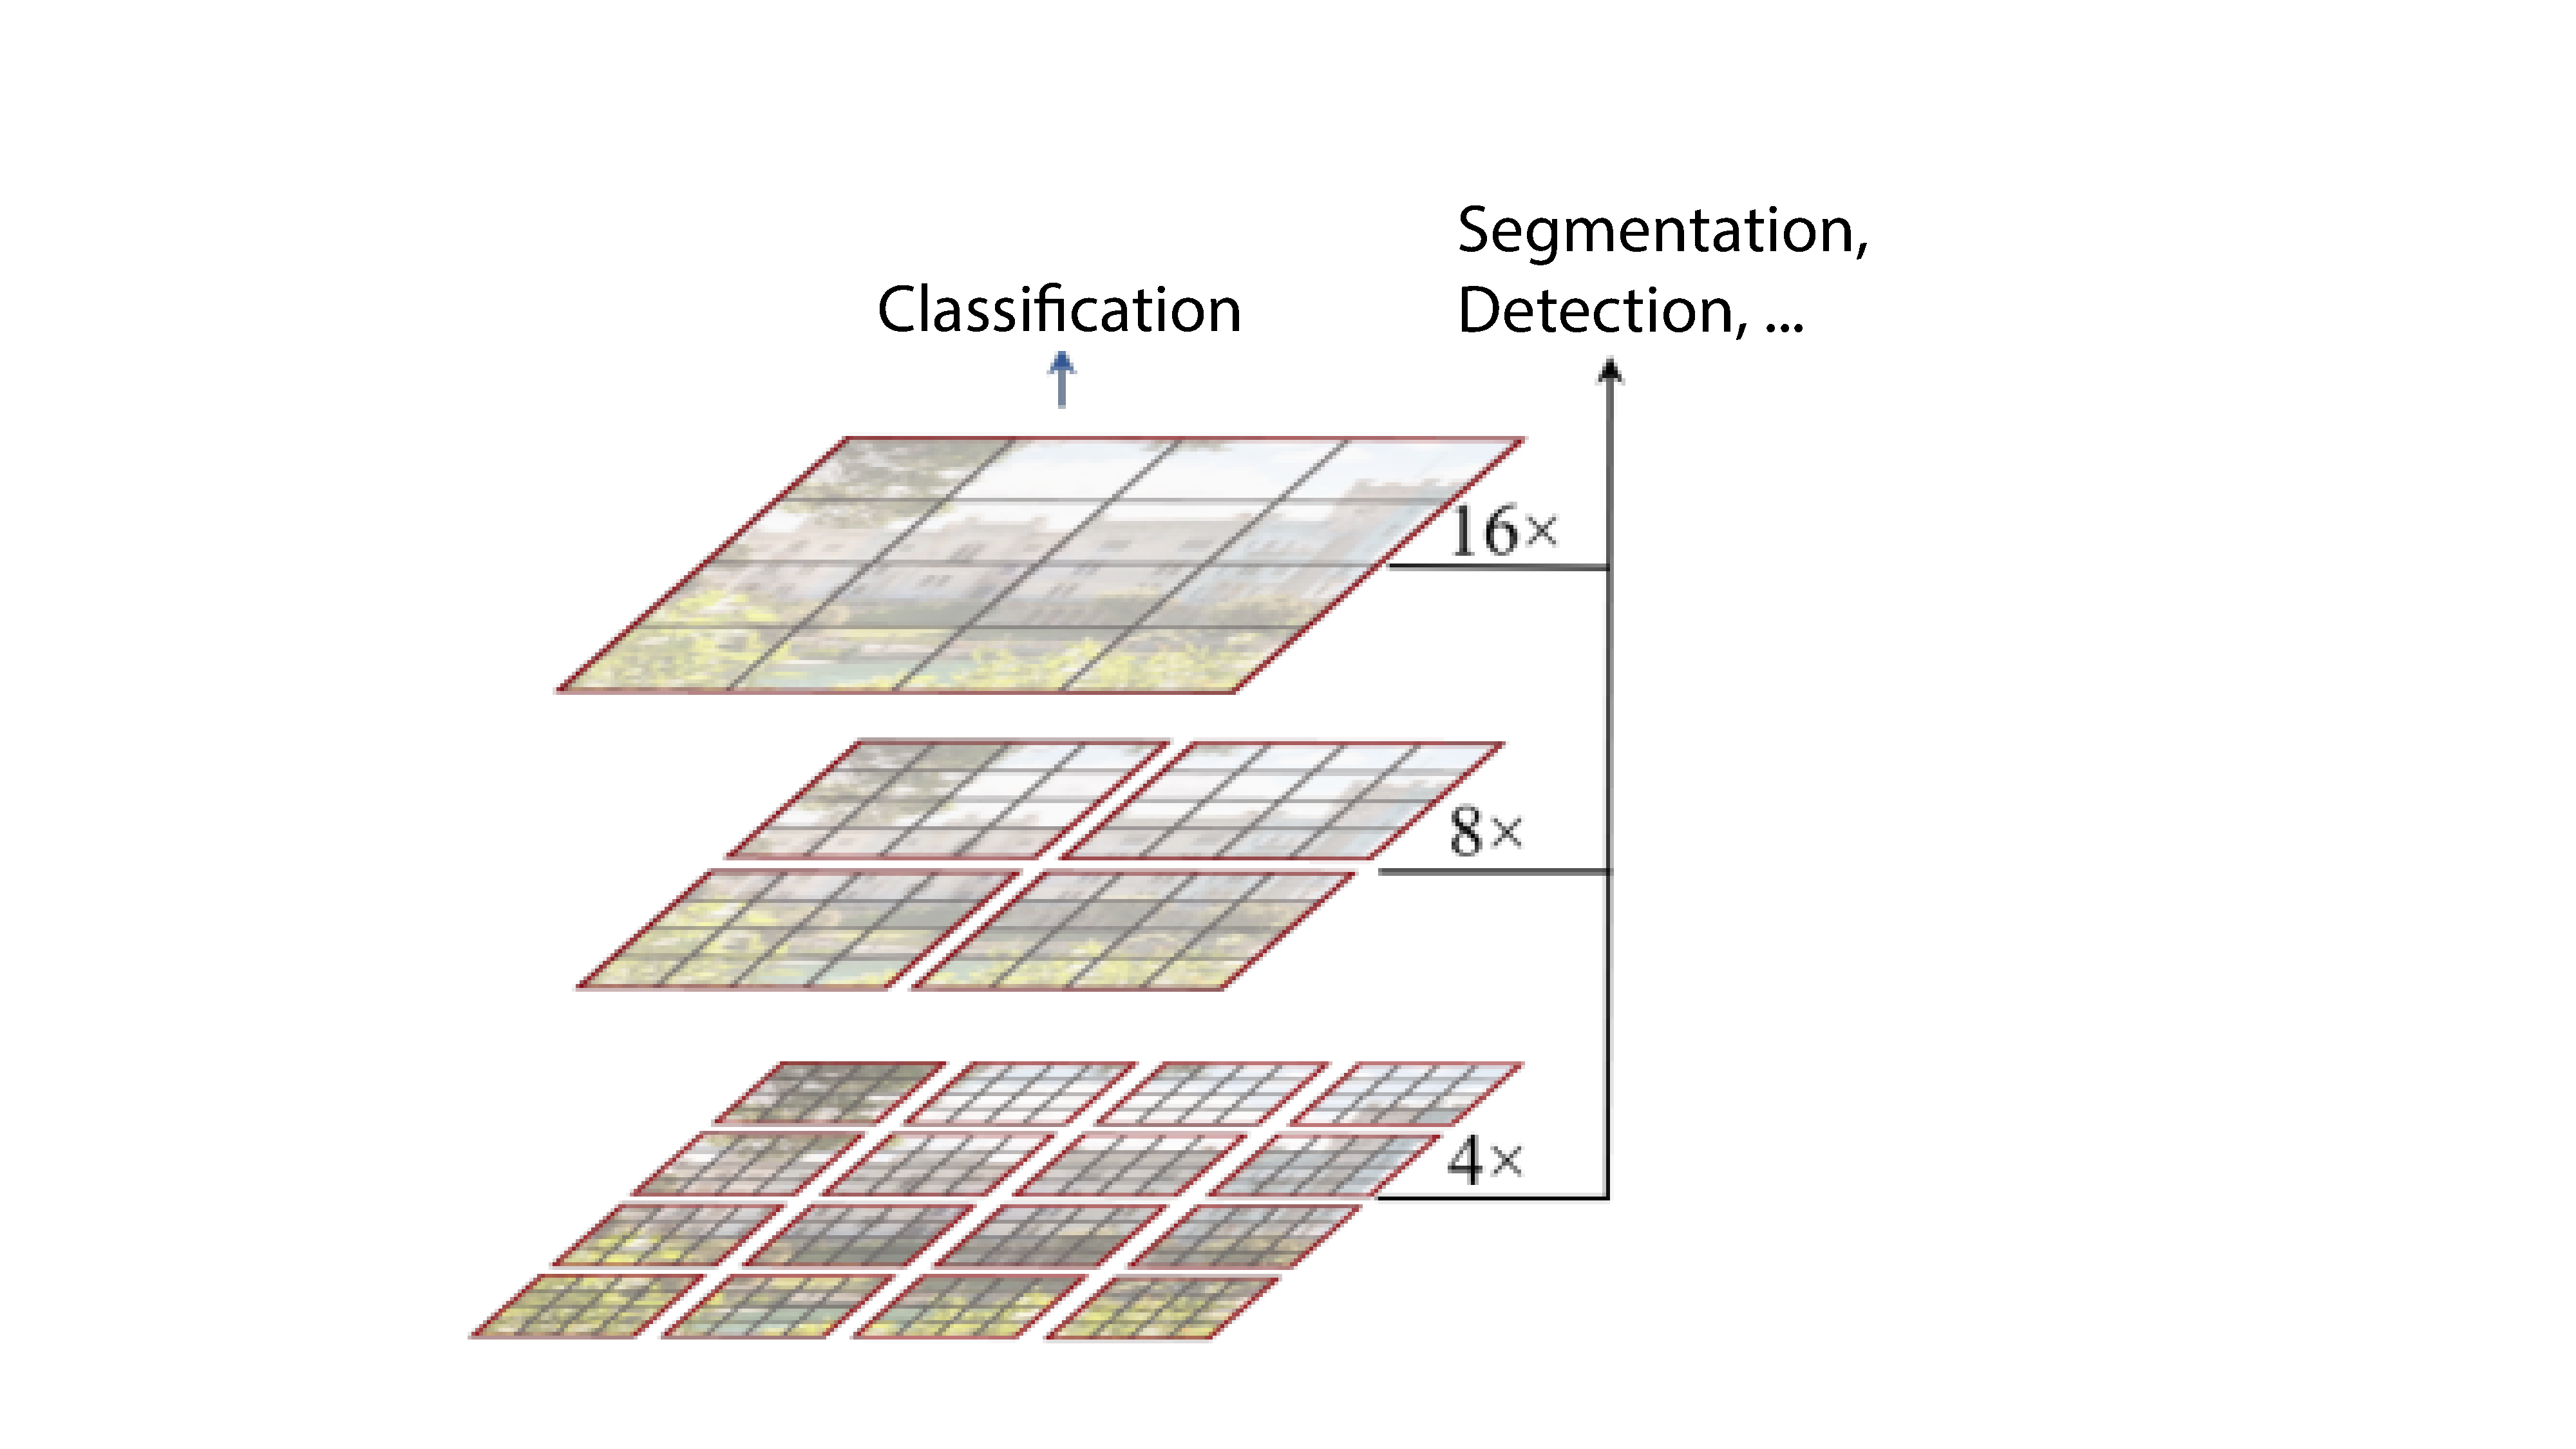
\includegraphics[width=\textwidth]{swin-vs-vit-archi-a.pdf}
                \caption{Swin Transformer}
                \label{fig:swin_transformer_data_flow}
            \end{subfigure}
            \hfill
            \begin{subfigure}[b]{0.45\textwidth}
                \centering
                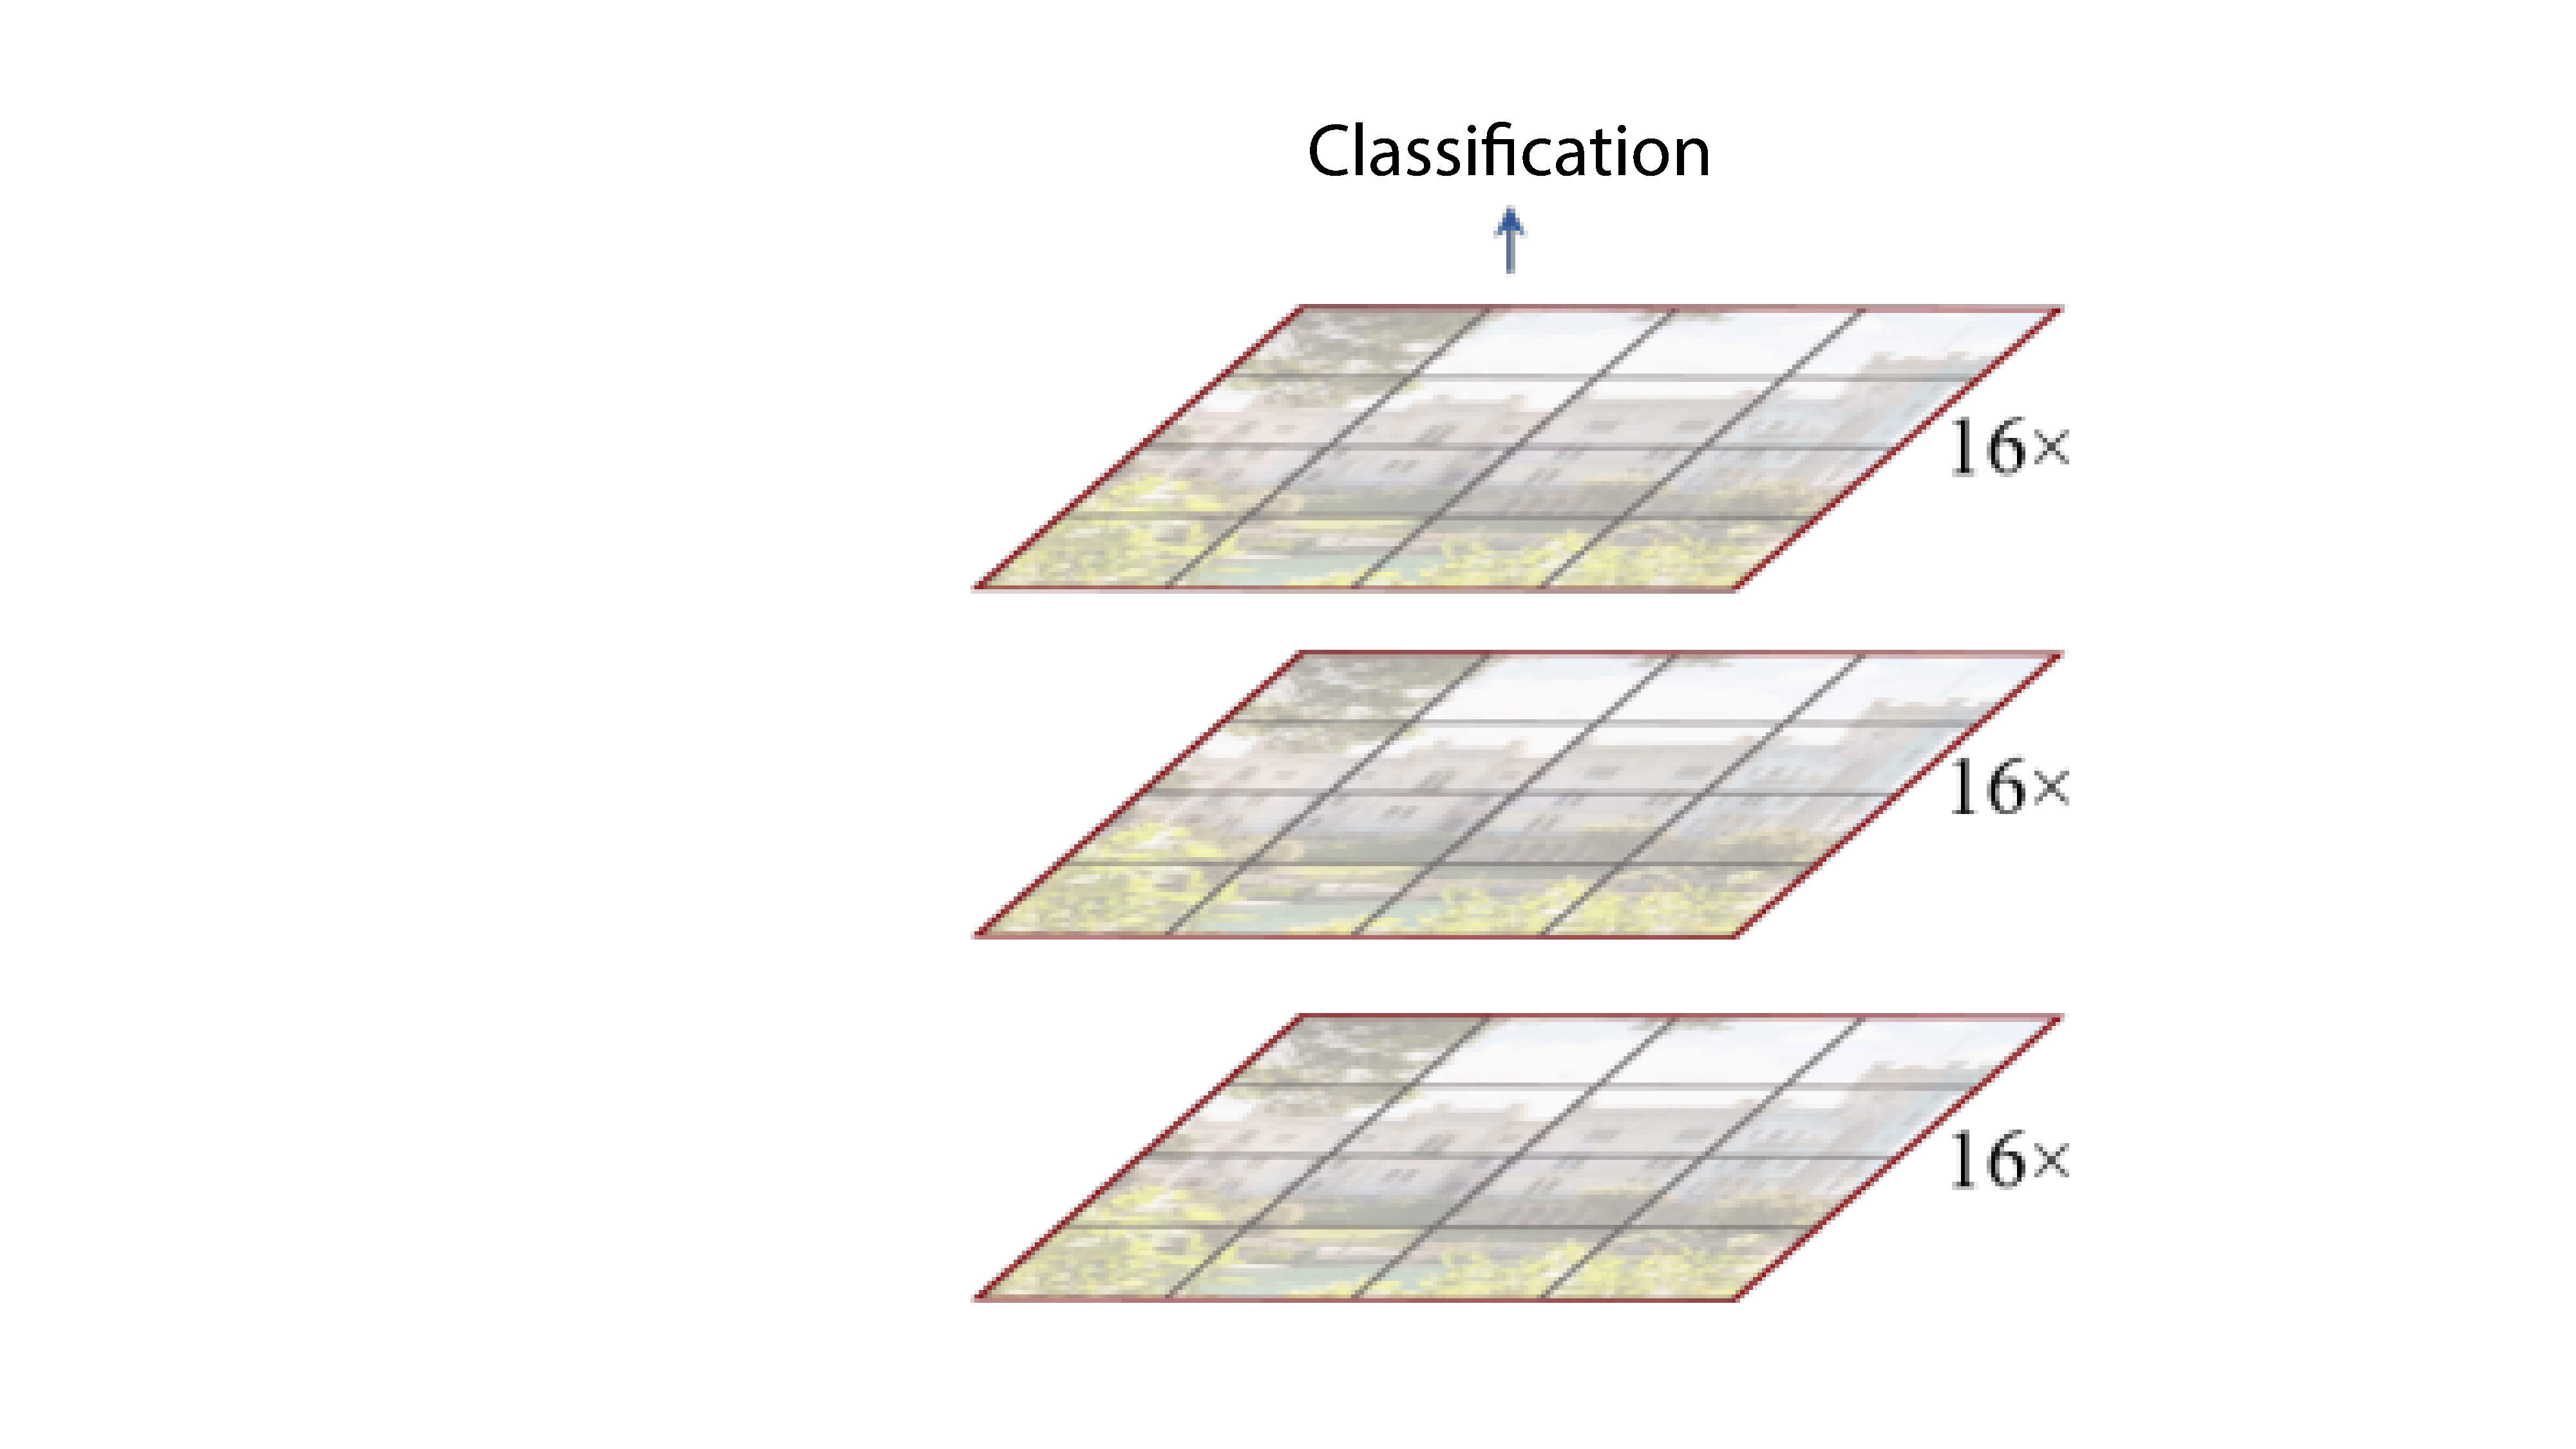
\includegraphics[width=\textwidth]{swin-vs-vit-archi-b.pdf}
                \caption{Vision Transformers}
                \label{fig:vit_data_flow}
            \end{subfigure}
        \end{minipage}
    }
    \caption{Comparison of Swin Transformer and ViT Architectures}
    \label{fig:swin_vs_vit_architecture}
\end{figure}

Because of the hierarchical nature of the Swin Transformer, it is particularly well-suited for tasks that require a combination of global context (to indentify the overall structure of the image) and local details (to capture fine-grained features, e.g., edges, textures). This makes it a strong candidate for image segmentation tasks.

Also, the Contrastive and Multi-Modal Learning capabilities of UniCL can be effectively combined with the Swin Transformer's hierarchical architecture to enhance the model's ability to learn rich and discriminative features from both image and text modalities. This combination allows for a more comprehensive understanding of the data, leading to improved performance.

Now, getting all the background information, we can proceed to the proposed methodology. The proposed methodology consists of several key components, including the backbone architecture, CAM generation, pseudo label generation, segmentation prediction, and refinement. Each component plays a crucial role in enhancing the overall performance of the model.
% \chapter{Proposed Methodology}
\label{chap:methodology}

In our proposed methodology, we aim to leverage the strengths of both the UniCL framework and the Swin Transformer architecture to enhance the performance of our model. The methodology is structured into several key components, each addressing a specific aspect of the overall process. The following sections provide a detailed overview of each component, including the backbone architecture, CAM generation, pseudo label generation, segmentation prediction, and refinement.

\section{Overview}
\label{sec:overview}
In this section, we provide a high-level overview of the proposed methodology. The methodology is designed to address the challenges of weakly supervised semantic segmentation (WSSS) by leveraging the strengths of multi-modal learning frameworks like UniCL and advanced vision architectures such as the Swin Transformer. The key components of the methodology include:

\begin{figure}
    \centering
    \fbox{\includegraphics[width=0.985\textwidth, height = 1.02\textwidth]{figures/ProposedArchitecture.pdf}}
    \caption{Architecture of \textit{UniCL-AffSeg}}
    \label{fig:architecture}
\end{figure}

\begin{itemize}
    \item \textbf{Feature Extraction from Backbone}: The backbone network is responsible for generating Class Activation Maps (CAMs) from input images. We experiment with UniCL as the backbone due to its multi-modal capabilities and state-of-the-art performance in generating high-quality CAMs.
    \item \textbf{CAM Generation}: CAMs are generated using Grad-CAM techniques adapted for multi-modal models like UniCL. These CAMs highlight the regions of interest in the image for each class.
    \item \textbf{Segmentation Prediction}: The feature maps from the backbone are aggregated and passed through a decoder to produce segmentation predictions. The decoder employs multi-head transformer layers to refine the predictions.
    \item \textbf{CAM Refinement and Pseudo-Label Generation}: Initial CAMs are refined using affinity-based techniques and random walk propagation to generate high-quality pseudo-labels. These pseudo-labels serve as supervision for training the segmentation model.
    \item \textbf{Loss Function}: A combination of segmentation loss and affinity loss is used to optimize the model. The affinity loss ensures consistency between the affinity maps of the decoder and the pseudo-labels, while the segmentation loss aligns the predictions with the refined CAMs.
\end{itemize}

The proposed methodology integrates these components into a cohesive framework, enabling the generation of accurate segmentation maps from weak supervision signals. \autoref{fig:architecture} illustrates the overall architecture of the proposed methodology, highlighting the flow of data through each component.


\section{Feature Extraction from Backbone}
\label{sec:feature_extraction_from_backbone}

In weakly supervised semantic segmentation (WSSS), two components play a crucial role: class activation maps (CAMs) and pseudo labels. The CAMs are first generated from the backbone network, and these are subsequently used to construct pseudo labels. The pseudo labels then serve as supervision for training the segmentation head—or the full segmentation model in the case of a multi-stage approach. 

The accuracy of the initial CAMs directly affects the quality of the pseudo labels and, consequently, the performance of the segmentation model. To achieve robust feature representations, we employ UniCL \cite{vl_unicl}, a multi-modal contrastive learning model built upon the CLIP framework. In this section, we first introduce CLIP, outlining its core architecture and characteristics. We then discuss UniCL and its innovations over CLIP, followed by a description of the Swin Transformer backbone that underpins the image encoding process.

\subsection{Contrastive Language-Image Pre-Training (CLIP)}
\label{subsec:clip}

CLIP \cite{vl_clip} is a multi-modal learning framework that utilizes contrastive learning to align images and text within a shared embedding space. It is designed to acquire representations that generalize well across different tasks without the need for task-specific fine-tuning. By training on extensive datasets of image-text pairs, CLIP learns to capture meaningful associations between visual and textual modalities.

\subsection{CLIP Architecture}
\label{subsec:clip_architecture}

\subsubsection{CLIP Components}
CLIP comprises two principal components:

\begin{itemize}
    \item \textbf{Image Encoder}: Responsible for processing images and extracting feature representations. This typically involves a Swin Transformer, pooling layers, and additional modules to capture spatial hierarchies and relationships within image data.
    \item \textbf{Text Encoder}: Processes textual data and converts it into a format suitable for comparison with image features. It generally includes transformer layers and attention mechanisms to capture semantic relationships within the text.
\end{itemize}

CLIP is trained using a contrastive loss function that aligns image and text features in a shared embedding space. This enables the model to learn representations applicable to a variety of tasks, such as image classification, object detection, and image segmentation. In the context of this work, CLIP's capabilities are leveraged for weakly supervised semantic segmentation, which relies solely on image-level classification.

\subsection{Characteristics of CLIP}
\subsubsection{Multi-Modal Learning}
\label{subsec:multi_modal_learning}
Multi-modal learning involves integrating information from different modalities, such as images and text, to enhance model performance. By combining complementary cues from multiple sources, models can develop a deeper and more comprehensive understanding of the data. For instance, in classification tasks, leveraging both visual and textual data enables the model to capture more nuanced semantic relationships. A key advantage of this approach is the potential for zero-shot learning, where the model can recognize and classify images from previously unseen categories. This is accomplished by aligning visual features with corresponding textual descriptions, allowing the model to generalize beyond the training set. Such capabilities are particularly valuable, as classification often underpins many downstream applications.

\subsubsection{Contrastive Learning}
\label{subsec:contrastive_learning}
Contrastive learning is a self-supervised approach focused on learning representations by distinguishing between positive and negative pairs. The objective is to bring representations of related inputs (such as an image and its corresponding textual description) closer in a shared embedding space, while pushing apart representations of unrelated inputs. This is typically achieved using a contrastive loss function, which minimizes the distance between positive pairs and maximizes it for negative pairs. Such a strategy enables models to acquire robust, discriminative, and generalizable feature representations.

\subsubsection{Training Strategy}
\label{subsec:training_strategy}
The training strategy for multi-modal learning generally integrates both supervised and self-supervised techniques. Models are trained on large-scale datasets containing paired samples from different modalities, facilitating the learning of meaningful representations through methods such as contrastive learning. Data augmentation is commonly applied to enhance the diversity and robustness of the learned features, thereby improving the model's generalization to unseen data.

\subsubsection{Task-Agnostic Learning}
\label{subsec:task_agnostic_learning}
Task-agnostic learning refers to the development of representations that are not specialized for a single task but are applicable across a range of downstream applications. This is accomplished by focusing on learning generalizable features through training on diverse datasets and leveraging multi-modal information. As a result, models can adapt their learned representations to various tasks, including image classification, object detection, and image segmentation. This adaptability makes task-agnostic learning a valuable approach for constructing versatile and reusable models.

\subsection{Unified Contrastive Learning (UniCL)}
\label{subsec:unicl}

UniCL, or Unified Contrastive Learning \cite{vl_unicl}, is a multi-modal learning framework that extends the ideas of CLIP by unifying different contrastive learning strategies within a single architecture. This enables more effective and flexible learning from multiple modalities.

UniCL \cite{vl_unicl} is more than a straightforward extension of CLIP; it introduces several important innovations to improve both performance and adaptability.

A key feature of UniCL is its unified approach to contrastive learning, integrating image-label and text-label associations into a joint image-label-text space. This unified framework allows the model to leverage more positive pairs during training. While CLIP treats only the provided image-text pair as a positive match, UniCL recognizes that multiple text descriptions or images can correspond to the same category. For instance, both "a photo of a cat" and "a photo of a kitten" may be valid positive pairs for an image of a cat. UniCL's contrastive loss encourages the model to learn similarities across all features sharing the same category, resulting in a more comprehensive and robust shared representation space for images and text.

\subsubsection{Unified Image-Text-Label Contrast in UniCL}
\label{subsec:unified_image_text_label_contrast}

UniCL employs a bidirectional learning objective between image-text pairs:
\begin{equation} \label{eq:unified_image_text_label_contrast}
    \min_{\{\theta, \phi\}} \mathcal{L}_{\text{BiC}} = \mathcal{L}_{i2t} + \mathcal{L}_{t2i},
\end{equation}
where \(\mathcal{L}_{i2t}\) and \(\mathcal{L}_{t2i}\) are the image-to-text and text-to-image contrastive losses, respectively. And \(\theta\) and \(\phi\) are the parameters of the image and text encoders, respectively.

To align the representations of images and their corresponding textual descriptions within a batch, the image-to-text contrastive loss is formulated by \cite{vl_unicl}. This loss encourages the model to associate each image with all relevant text features that share the same class label, thereby strengthening the alignment between visual and textual modalities in the shared embedding space:
\begin{equation} \label{eq:unicl_image_to_text_contrastive_loss}
    \mathcal{L}_{i2t} = - \sum_{i \in \mathcal{B}} \frac{1}{|\mathcal{P}(i)|} \sum_{k \in \mathcal{P}(i)} 
    \log \frac{\exp(\tau \mathbf{u}_i^\top \mathbf{v}_k)}{\sum_{j \in \mathcal{B}} \exp(\tau \mathbf{u}_i^\top \mathbf{v}_j)},
\end{equation}
where $k \in \mathcal{P}(i) = \{k | k \in \mathcal{B}, y_k = y_i\}$, i.e., the set of all images in the batch that belong to the same class as image $i$.

Conversely, the text-to-image contrastive loss, which aligns each text feature in a batch with its corresponding image features, is formulated as:

\begin{equation} \label{eq:unicl_text_to_image_contrastive_loss}
    \mathcal{L}_{t2i} = - \sum_{j \in \mathcal{B}} \frac{1}{|\mathcal{P}(j)|} \sum_{k \in \mathcal{P}(j)} 
    \log \frac{\exp(\tau \mathbf{u}_k^\top \mathbf{v}_j)}{\sum_{i \in \mathcal{B}} \exp(\tau \mathbf{u}_i^\top \mathbf{v}_j)},
\end{equation}
where $k \in \mathcal{P}(j) = \{k \mid k \in \mathcal{B}, y_k = y_j\}$, i.e., the set of all text features in the batch that belong to the same class as text $j$.

\subsubsection{Comparison with CLIP}
\label{subsec:clip_vs_unicl}

In case CLIP \cite{vl_clip}, for an image, there is only one positive text feature. In other words, $\mathcal{P}(i) = {i} \in \mathcal{B}$; and $\mathcal{P}(j) = {j} \in \mathcal{B}$. So, the image-to-text contrastive loss is defined as:

\begin{equation} \label{eq:clip_image_to_text_contrastive_loss}
    \mathcal{L}_{i2t} = - \sum_{i \in \mathcal{B}} 
    \log \frac{\exp(\tau \mathbf{u}_i^\top \mathbf{v}_i)}{\sum_{j \in \mathcal{B}} \exp(\tau \mathbf{u}_i^\top \mathbf{v}_j)},
\end{equation}
where $i \in \mathcal{B}$ is the index of the image in the batch.

And the text-to-image contrastive loss is defined as:

\begin{equation} \label{eq:clip_text_to_image_contrastive_loss}
    \mathcal{L}_{t2i} = - \sum_{j \in \mathcal{B}} 
    \log \frac{\exp(\tau \mathbf{u}_j^\top \mathbf{v}_j)}{\sum_{i \in \mathcal{B}} \exp(\tau \mathbf{u}_i^\top \mathbf{v}_j)},
\end{equation}
where $j \in \mathcal{B}$ is the index of the text feature in the batch. 

The equations \ref{eq:unified_image_text_label_contrast}-\ref{eq:clip_text_to_image_contrastive_loss} are taken from \cite{vl_unicl}.

This means that $\mathcal{L}_{BiC}$ becomes CLIP training objective. The main property in \autoref{eq:unicl_text_to_image_contrastive_loss} is that for each image feature, any of the text features in the batch can be used as a positive pair. And so is the case for \autoref{eq:unicl_text_to_image_contrastive_loss}.

Second, UniCL replaces CLIP's ViT backbone with a Swin Transformer \cite{transformer_swin} backbone. The Swin Transformer is a hierarchical vision transformer that captures both local and global information in images, making it more suitable for various vision tasks.

\subsection{Swin Transformer}
\label{subsec:swin_transformer}
The Swin Transformer \cite{transformer_swin} is a hierarchical vision transformer architecture that utilizes a shifted windowing mechanism to effectively capture both local and global image information. It is engineered for computational efficiency while delivering strong performance across a range of computer vision tasks. The model is organized into multiple stages, each comprising distinct transformer blocks, which enables the processing of images at varying resolutions and facilitates the extraction of multi-scale features.

\autoref{fig:swin_vs_vit_architecture} presents a comparative overview of the Swin Transformer and Vision Transformer (ViT) architectures. The principal difference between the two lies in their respective processing paradigms: the Swin Transformer adopts a hierarchical framework, operating on feature maps at multiple scales, whereas ViT processes the entire image globally at a single resolution. This hierarchical design empowers the Swin Transformer to simultaneously capture fine-grained local details and broader contextual information, making it particularly advantageous for applications that demand both.

Within the Swin Transformer, hierarchical feature maps are constructed by progressively merging image patches (shown in gray) at deeper network layers. Self-attention is computed exclusively within localized windows (indicated in red), resulting in linear computational complexity with respect to the input image size. This approach not only enhances efficiency but also renders the Swin Transformer highly suitable for dense prediction tasks, such as image segmentation and classification.

Conversely, conventional vision transformers like ViT generate feature maps at a single, lower resolution and apply self-attention globally, which incurs quadratic computational complexity relative to the input size. While global attention can be beneficial for certain tasks, it is less efficient for dense recognition scenarios compared to the localized attention employed by the Swin Transformer.

\begin{figure}[htbp]
    \centering
    \fbox{ % Draw a box around the entire figure
        \begin{minipage}{0.95\textwidth} % Adjust the width as needed
            \begin{subfigure}[b]{0.49\linewidth}
                \centering
                \caption{Swin Transformer}
                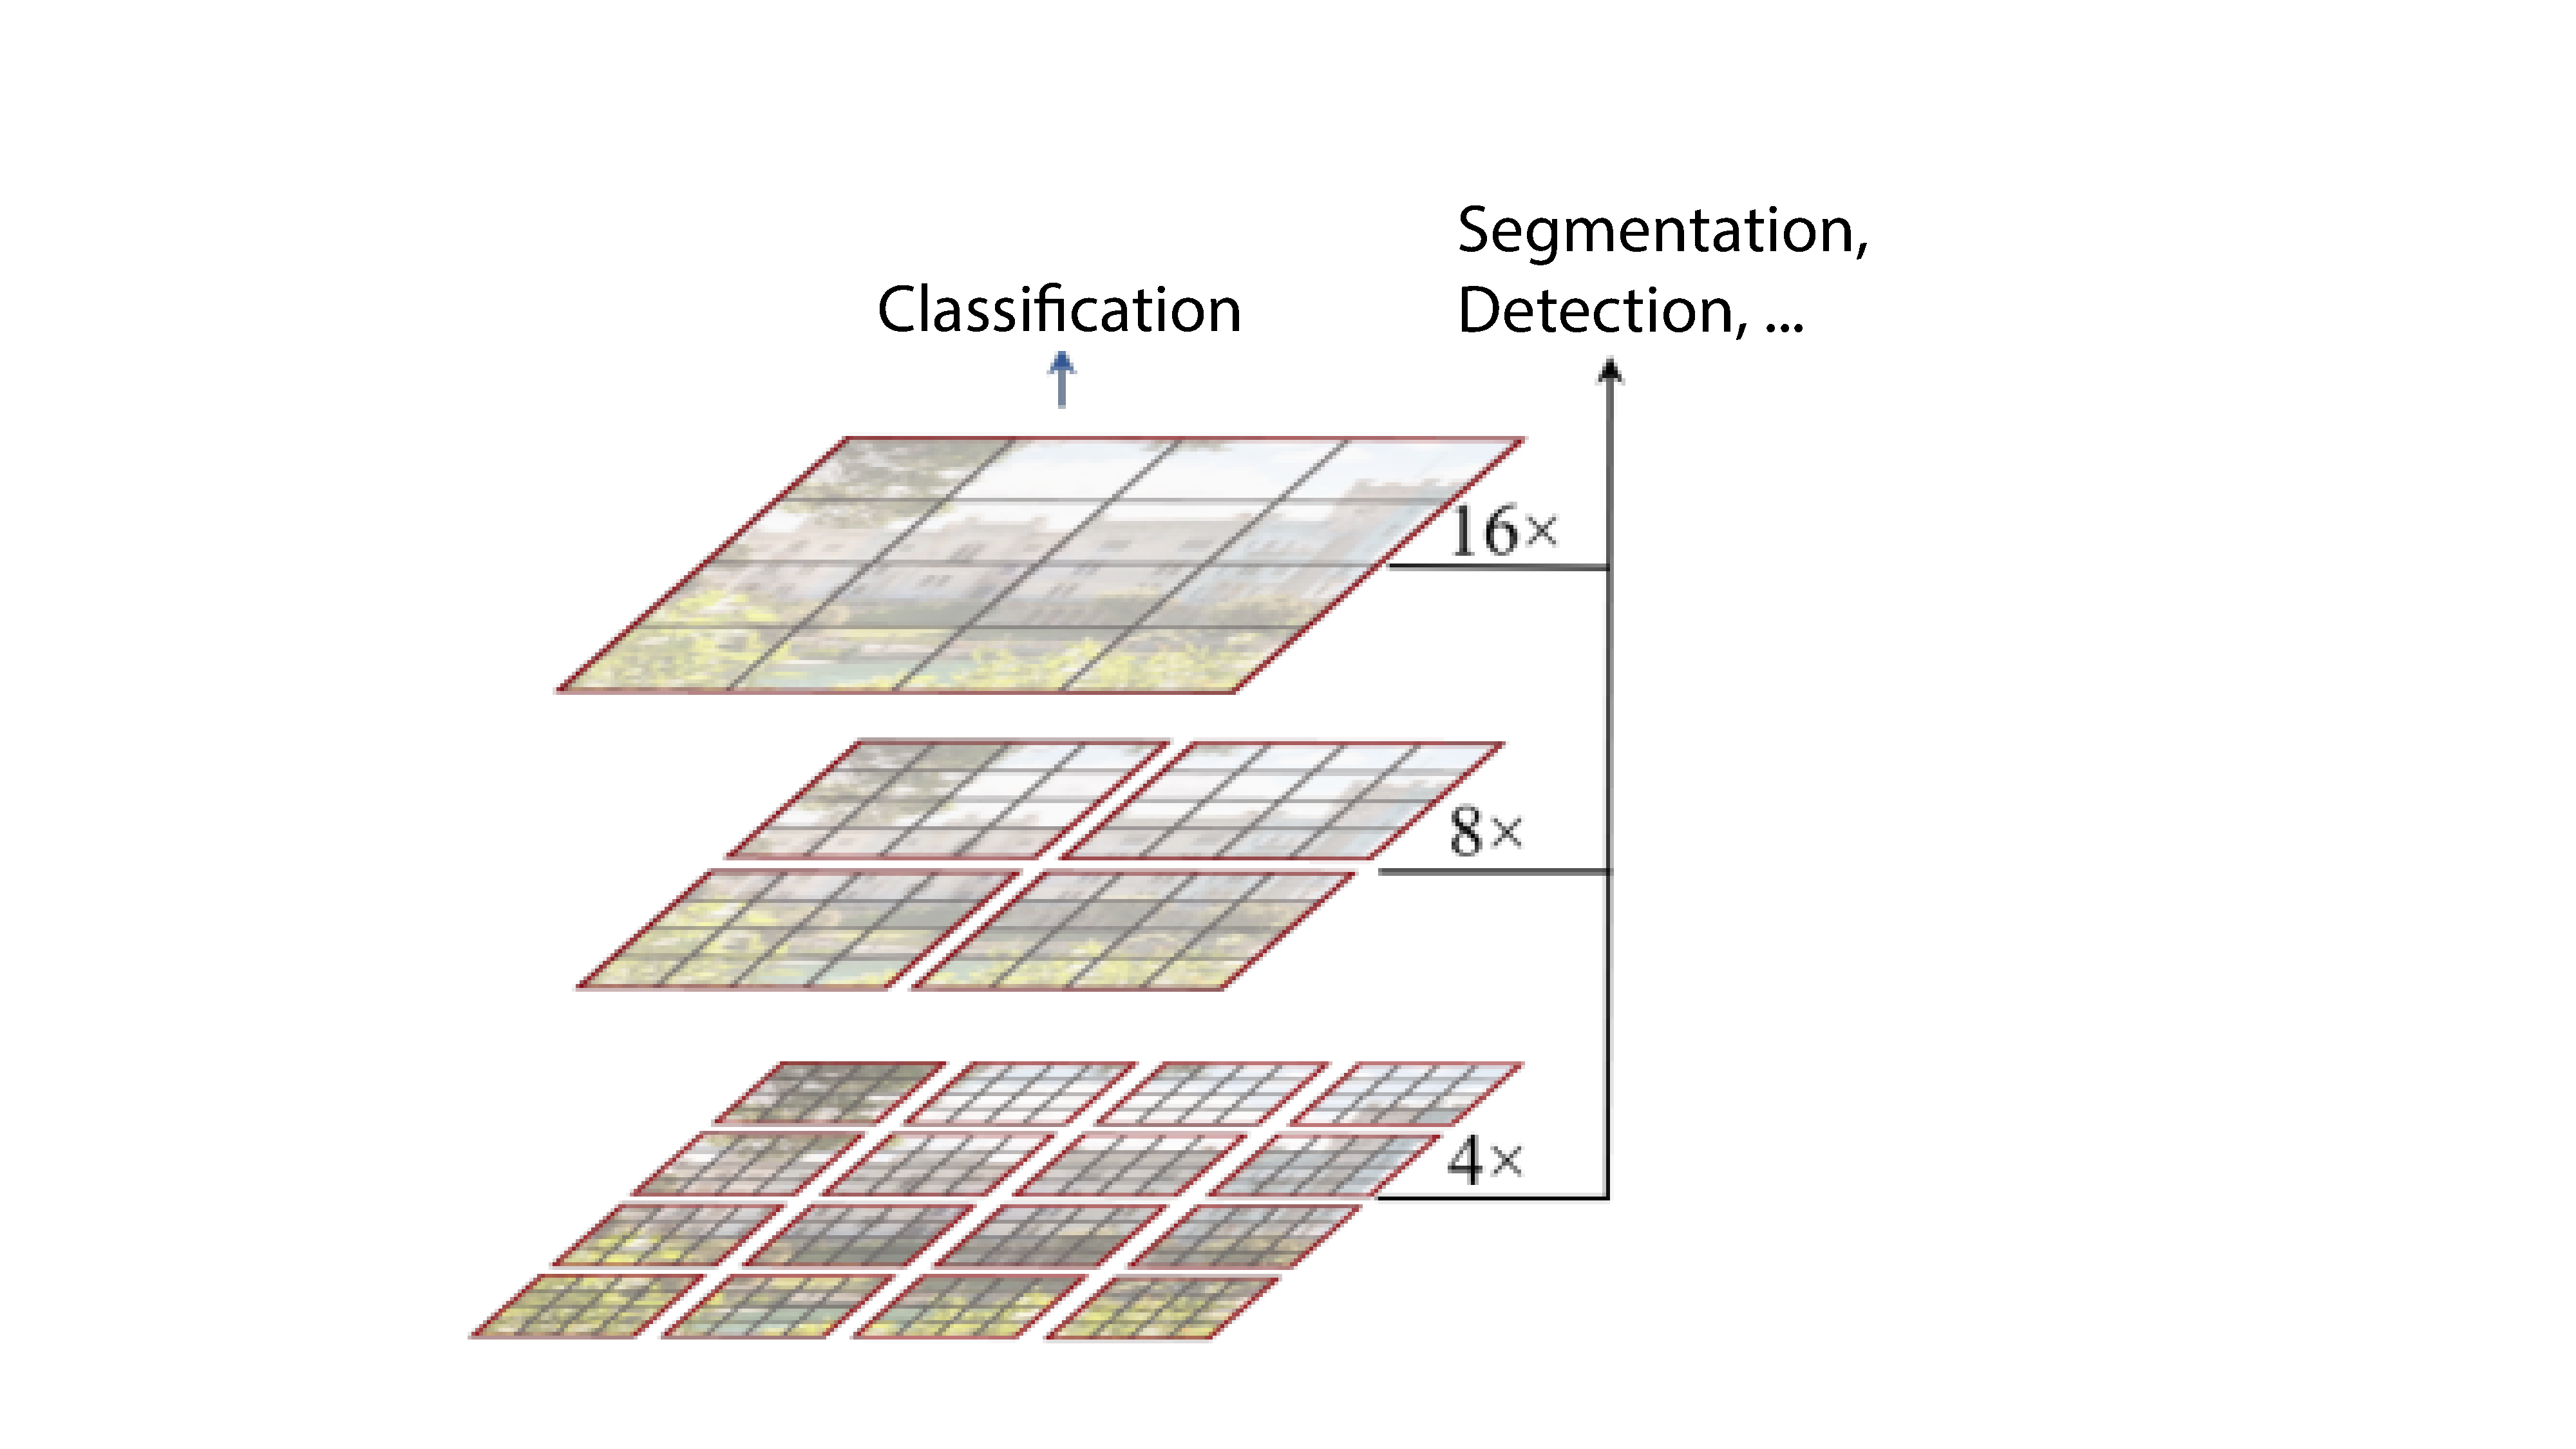
\includegraphics[width=\textwidth]{swin-vs-vit-archi-a.png}
                \label{fig:swin_transformer_data_flow}
            \end{subfigure}
            \hfill
            \begin{subfigure}[b]{0.4\linewidth}
                \centering
                \caption{Vision Transformers}
                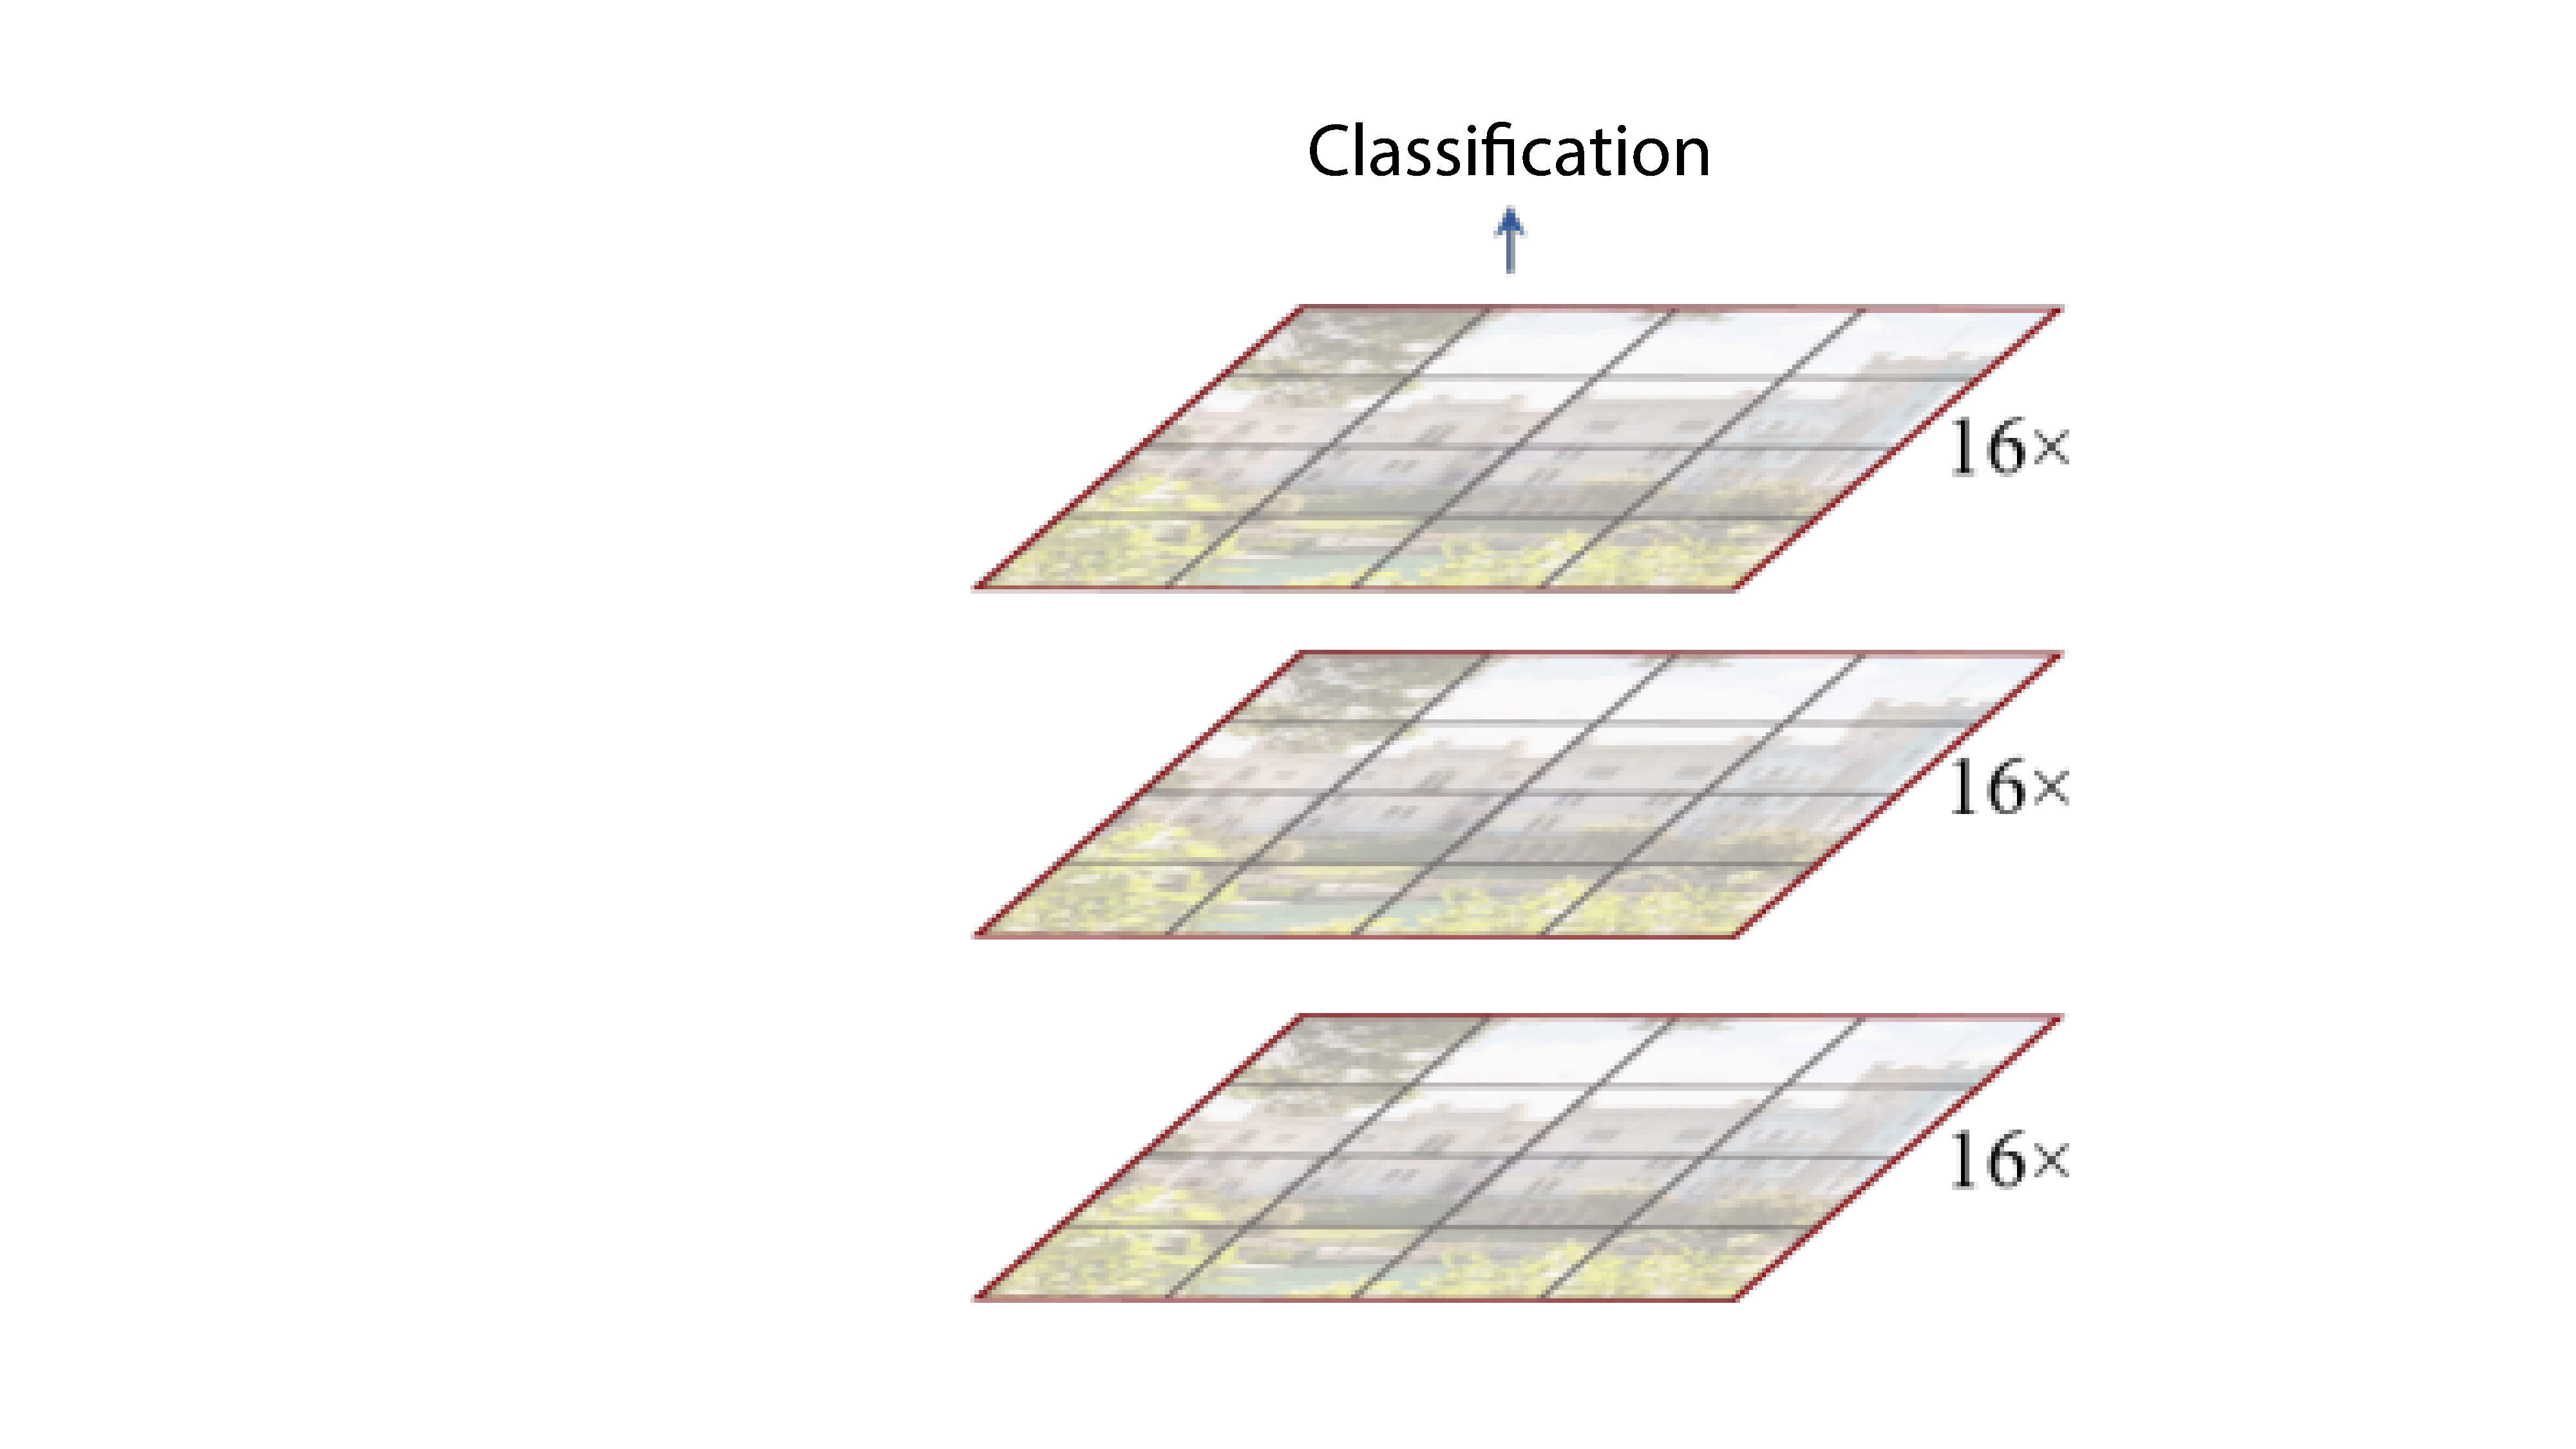
\includegraphics[width=\textwidth]{swin-vs-vit-archi-b.png}
                \label{fig:vit_data_flow}
            \end{subfigure}
        \end{minipage}
    }
    \caption{Comparison of Swin Transformer \cite{transformer_swin} and ViT \cite{transformer_vit} Architectures. Image taken from \cite{transformer_swin}.}
    \label{fig:swin_vs_vit_architecture}
\end{figure}

Owing to its hierarchical structure, the Swin Transformer is exceptionally well-suited for tasks that necessitate the integration of global context—essential for discerning the overall image structure—and local information, which is critical for identifying intricate features such as edges and textures. This makes it a compelling choice for image segmentation applications.

Furthermore, integrating the contrastive and multi-modal learning strengths of UniCL with the Swin Transformer's hierarchical design can significantly enhance the model's capacity to learn robust and discriminative representations from both visual and textual data. This synergy facilitates a more holistic understanding of multimodal inputs, thereby improving overall model performance.

With this foundational context established, the subsequent section details the proposed methodology, which comprises several core components: the backbone architecture, class activation map (CAM) generation, pseudo-label creation, segmentation prediction, and refinement. Each of these elements is integral to optimizing the model's effectiveness.


\begin{figure}[ht]
    \centering
    \setlength{\tabcolsep}{2pt} % adjust spacing
    \renewcommand{\arraystretch}{0.9}
    \fbox{ % Add border around the figure
        \begin{minipage}{0.6\textwidth}
            \centering
            % CAMs with class labels on the left
            \begin{tabular}{c c} % first column = label

            % Column headers
            (a) Original Image & (b) CAM \\
            [1mm]
            \includegraphics[width=0.45\textwidth,height=0.45\textwidth]{figures/originals/2009_004084.jpg}
            & 
            \includegraphics[width=0.45\textwidth,height=0.45\textwidth]{figures/test_cams/ours/2009_004084_2.jpg}
            \\
            \end{tabular}
        \end{minipage}
    }
    \caption{Original image and CAM generated by our method for class \textit{Bird}.}
    \label{fig:cam_examples}
\end{figure}

\section{CAM Generation}
\label{sec:cam_generation}

\autoref{fig:cam_generation_process_clip} shows the process of generating CAMs using CLIP/UniCL. We have used Grad-CAM. The process is similar to the method discussed in \autoref{subsec:grad_cam}, which is used to generate CAMs using CNN-based models.
 But there are some differences.

AS CLIP is a multi-modal model, the main classification task is to find similarity between the image and text. If we want to generate the CAM for $N$ classes, we need to provide $N$ text features as input. So, at the very beginning, we need to encode the text features using the CLIP text encoder, and store them.

An MLP layer takes the linear combination of the input features and the weights. We do the same thing when finding similarity score between the image and text features, take the linear combination of the image features and the text features. So, we can consider these text features as the "neuron weights" of the classifier head.

Then, we need to pass the image through the CLIP image encoder to get the feature maps. The rest of the process is the same as Grad-CAM. An example of the produced CAM for the \textit{Motorbike} class is shown in \autoref{fig:cam_examples}.


\begin{figure}[htbp]
    \centering
    \fbox{\includegraphics[width=0.8\textwidth]{methodology_cam.pdf}}
    \caption{CAM Generation Process using UniCL}
    \label{fig:cam_generation_process_clip}
\end{figure}

\section{Segmentation Prediction}
\label{sec:segmentation_prediction}
The segmentation prediction module is responsible for producing pixel-level class predictions for the input image. It comprises two primary stages: aggregation of encoder features and a decoder built with multi-head transformer layers. The design is inspired by the approach in \cite{wsss_frozen_clip}.

\subsection{Encoder Feature Aggregation}
\label{subsec:en_feature_agg}
In accordance with the methodology outlined in \cite{wsss_frozen_clip}, the feature representations extracted from each transformer block of the UniCL image encoder \cite{vl_unicl} are forwarded to the decoder for further processing. Denote the output feature map from the $l$-th transformer block as \( F_l^{\text{init}} \), where \( l = 1, \dots, N \). To harmonize the feature dimensions and enhance representational capacity, each \( F_l^{\text{init}} \) is individually transformed via a dedicated multilayer perceptron (MLP). Specifically, the transformation is defined as:
\begin{equation}
    F_l^{\text{new}} = W_{1}^{\text{fc}} \left( \text{ReLU} \left( W_{2}^{\text{fc}}(F_l^{\text{init}}) \right) \right),
\end{equation}
where \( W_{1}^{\text{fc}} \) and \( W_{2}^{\text{fc}} \) denote learnable fully connected layers, and \(\text{ReLU}(\cdot)\) represents the rectified linear unit activation function. This procedure ensures that the multi-scale features from different encoder stages are suitably projected for subsequent aggregation and decoding.


After that, all new feature maps \( F_l^{\text{new}} \) for \( l = 1, \dots, N \) are concatenated together, which are then processed by a convolution layer to generate a fused feature map \( F_u \) \cite{wsss_frozen_clip}:
\begin{equation}
    F_u = \text{Conv}\left( \text{Concat}\left[ F_1^{\text{new}}, F_2^{\text{new}}, \dots, F_N^{\text{new}} \right] \right),
    \tag{2}
\end{equation}

where \( F_u \in \mathbb{R}^{d \times h \times w} \), and \( d \), \( h \), and \( w \) represent the channel dimension, height, and width of the feature map, respectively. \(\text{Conv}(\cdot)\) is a convolutional layer, and \(\text{Concat}[\cdot]\) denotes the concatenation operation.


\subsection{Generating Final Prediction}
\label{subsec:decoder_final_pred}

Several sequential multi-head transformer layers are designed to generate the final prediction \( P \) \cite{wsss_frozen_clip}:
\begin{equation}
    \label{eq:prediction}
    P = \text{Conv}(\phi(F_u)) \uparrow,
\end{equation}
where \( P \in \mathbb{R}^{C \times H \times W} \), \( C \) is the number of classes including background, and \(\phi\) represents the sequential multi-head transformer blocks [12]. Each transformer block contains a multi-head self-attention module, a feed-forward network, and two normalization layers. The operator \(\uparrow\) denotes an upsampling operation to align the prediction map size with the original image.


\section{CAM Refinement and Pseudo-Label Generation}
\label{sec:refinement}
\subsection{Affinity based CAM refinement}  
The initial CAMs produced by the backbone tend to focus only on sparse, highly discriminative regions. These activations are often noisy and insufficient to be used directly as supervision. Therefore, a refinement module is required where the initial CAM is improved. The refined CAM is then used as a pseudolabel for supervision.  

The most common strategy for rectifying CAMs is by exploiting the feature relationships within the backbone that generates them. This is referred to as affinity-based CAM refinement, first introduced by \cite{wsss_affinitynet}. In transformer-based backbones, the attention maps naturally encode semantic-level affinities between tokens or patches. From these attention maps, an affinity matrix $A_f$ can be constructed and employed for CAM refinement via random walk propagation. In parallel, another affinity matrix, $A$, can be derived from the predicted pseudolabel produced by the decoder. The cross-entropy loss between these two affinity matrices is then incorporated into the training objective.  

However, in our case, the backbone responsible for generating the CAMs is \textbf{frozen}, meaning that its attention maps remain fixed and do not update during training. To address this limitation, Frozen CLIP \cite{wsss_frozen_clip} proposes utilizing the affinity derived from intermediate features of the encoder instead of directly relying on the backbone's frozen attention. The backbone attention maps are then used only to influence this encoder-derived affinity, producing a final refined matrix $R$, which is further transformed into a transition matrix $T$ for random walk propagation.  

\begin{figure}[t]
    \centering
    \fbox{\includegraphics[width=0.9\textwidth]{figures/DecoderRFM}}
    \caption{Decoder and Refinement Module}
    \label{fig:decoder}
\end{figure}

In our setup, the UniCL backbone is based on the Swin Transformer, whose shifted-window design restricts the attention mechanism to \textbf{local regions}. Consequently, the attention maps fail to capture the \textbf{global semantic affinities} necessary for effective CAM propagation, and we could not use them directly for refinement. To overcome this, we compute affinities from the \textbf{intermediate feature maps of the Swin encoder}.  

Formally, let $f^{(k)} \in \mathbb{R}^{C \times L}$ denote the feature map from the $k$-th encoder block, where $C$ is the channel dimension and $L = h \times w$ represents the flattened spatial resolution. Each feature map is first normalized along the channel dimension:

\begin{equation}
\tilde{f}^{(k)}_i = \frac{f^{(k)}_i}{\| f^{(k)}_i \|_2}, \quad i = 1, \dots, L
\end{equation}

The affinity between spatial positions $i$ and $j$ within block $k$ is then computed as the dot-product similarity:

\begin{equation}
A^{(k)}_{ij} = \tilde{f}^{(k)}_i{}^\top \tilde{f}^{(k)}_j
\end{equation}

We compute such affinity matrices across multiple intermediate encoder blocks to capture complementary semantic relations at different abstraction levels. The resulting set of affinities is represented as:

\begin{equation}
\mathcal{A} = \{ A^{(1)}, A^{(2)}, \dots, A^{(N)} \}, \quad \mathcal{A} \in \mathbb{R}^{N \times hw \times hw}
\end{equation}

This multi-block affinity representation provides richer contextual cues for propagating and refining class activation maps.


\subsection{Extracting affinity map from the decoder}
\label{subsec:decoder_aff_mat}
Based on the feature map $F_u$ obtained from the decoder (as defined in Eq.~(2)), an affinity map is constructed as follows:

\begin{equation}
    \label{eq: A_f}
    A_f = \text{Sigmoid}(F_u^\top F_u),
\end{equation}

where $F_u \in \mathbb{R}^{d \times h \times w}$ is reshaped into a matrix of size $d \times hw$ before the computation. The $\text{Sigmoid}(\cdot)$ function ensures that the values in the resulting affinity map lie in the range $[0, 1]$. Consequently, the computed affinity map $A_f$ has the dimensions $\mathbb{R}^{hw \times hw}$. Here, $\top$ denotes the matrix transpose.

\subsection{Selecting affinity maps of the image encoder}
\label{subsec:att_map_encoder}
Following \cite{wsss_frozen_clip}, we extract all the affinity maps from the frozen CLIP image encoder, denoted as $\{A^l\}_{l=1}^N$, where each affinity map $A^l \in \mathbb{R}^{hw \times hw}$. To evaluate the reliability of each affinity map $A^l$, we compare it with the previously computed decoder affinity map $A_f$ using the following deviation score:

\begin{equation}
    S^l = \sum_{i=1}^{hw} \sum_{j=1}^{hw} \left| A_f(i, j) - A^l(i, j) \right|,
\end{equation}

where $S^l$ quantifies how much the affinity map (encoder) $A^l$ deviates from the reference affinity (decoder) $A_f$.  

Based on this score, we assign a binary weight $G^l$ to each affinity map:  

\begin{equation}
    G^l =
    \begin{cases}
        1, & \text{if } S^l < \dfrac{1}{N - N_0 + 1} \sum_{m=N_0}^N S^m, \\[8pt]
        0, & \text{otherwise}.
    \end{cases}
\end{equation}

Here, $G^l \in \{0,1\}$ is expanded to $G^l_e \in \mathbb{R}^{hw \times hw}$ for subsequent operations. The threshold is chosen as the average of the scores $\{S^m\}_{m=N_0}^N$ from the later layers of the encoder. If $S^l$ is lower than this threshold, the corresponding affinity map is considered reliable and retained ($G^l = 1$); otherwise, it is filtered out ($G^l = 0$).  

This selection mechanism ensures that only high-quality affinity maps consistent with the encoder-derived relationships are preserved, thereby improving the robustness of the CAM refinement process.  

\subsection{Utilizing the frozen encoder affinity maps}
\label{subsec: mul_attn_and_aff}
Using the affinity map $A_f$ and the filtered affinity maps of the encoder, we construct a refining map $R$ by weighing the decoder affinity matrix with the mean of the selected encoder affinity maps. This method of selection is adopted first by \cite{wsss_frozen_clip}. The equation is given as:

\begin{equation}
    R = A_f \odot \frac{ \sum_{l=1}^N G^l_e A^l}{N_m},
\end{equation}

where $\odot$ denotes element-wise multiplication, and $N_m$ is the number of valid encoder affinity maps that have passed the filtering stage, defined as:

\begin{equation}
    N_m = \sum_{l = N_0}^N G^l.
\end{equation}

Here, $G^l_e \in \mathbb{R}^{hw \times hw}$ is the expanded binary filter corresponding to $G^l$. The refining map $R$ effectively integrates the reliable encoder affinity maps weighted by the affinity map $A_f$, enhancing meaningful relationships while suppressing noisy or irrelevant information.

\subsection{Constructing the semantic transition matrix}
\label{subsec:trans_mat}
Now that we have the affinity matrix $R$, to apply the random walk propagation, we need to at first normalize the rows for converting it into a transition probability matrix. In addition, column normalization ensures consistency and symmetric behavior. Sinkhorn normalization \cite{math_sinkhorn} is thus used to convert $R$ into a double stochastic matrix $R_{\text{nor}}$.

Next, $R_{\text{nor}}$ is converted into a symmetric matrix by adding its transpose and normalizing the sum:

\[
    T = \frac{R_{\text{nor}} + R_{\text{nor}}^T}{2}, \quad \text{where} \quad R_{\text{nor}} = \text{Sinkhorn}(R)
\]

The matrix $T$ is now symmetric whose rows and columns are normalized. This is the transition probability matrix to be used for random walk.


\begin{figure}[tbp]
    \centering
    \fbox{\includegraphics[width=0.95\textwidth]{figures/RFM}}
    \caption{CAM refinement by exploiting affinity map}
    \label{fig:refinement}
\end{figure}

\subsection{Random Walk Propagation}
\label{subsec:random_walk}

The refined class activation map (CAM) for a specific class $c$, denoted as $M^c_f$ is found by random walk propagation as follows:

\begin{equation}
    M_f^c = B^c \odot T^\alpha \cdot M_{\text{init}}^c
\end{equation}

where, $M^c_{\text{init}} \in \mathbb{R}^{hw \times 1}$ is the initial CAM for class $c$, reshaped into vector form. $T$ is the transition probability matrix, $\alpha$ is the hyperparameter that controls the strength of the refinement we want to apply. It is equivalent to the number of iterations of the random walk propagation. \( B^c \in \mathbb{R}^{1 \times hw} \) is the box mask obtained from the CAM of class \( c \), and \( \odot \) denotes the Hadamard product. This masking is needed to restrict the refining region spatially. It is obtained for each target class c by thresholding the CAM of this class by a constant. The connected regions of the mask map are found and covered by minimum rectangle bounding boxes. These boxes mask the affinity of distant pixels, preventing over-expansion.

Finally, the refined CAM $M^c_f$ is passed through an online post-processing module - specifically, the pixel-adaptive refinement module proposed in \cite{wsss_afa_affinity_from_attention}.

\subsection{Pixel Adaptive refinement module}
\label{subsec:par}
To ensure local consistency, pixel-adaptive convolution is introduced by \cite{wsss_afa_affinity_from_attention}. It uses local RGB and spatial information to define the low-level pair-wise semantic affinity of two pixels. Given an input image \( I \in \mathbb{R}^{h \times w \times 3} \), the pairwise affinities between two pixels at positions \((i, j)\) and \((k, l)\) is calculated as follows:

- \( \kappa^{\text{rgb}}_{ij,kl} \) measures color similarity (the closer the colors, the higher the affinity).

- \( \kappa^{\text{pos}}_{ij,kl} \) measures spatial closeness (pixels closer in space have higher affinity).

These are defined as:

\[
    \kappa^{\text{rgb}}_{ij,kl} = -\frac{\| I_{ij} - I_{kl} \|^2}{w_1 \sigma^2_{\text{rgb}}}, \quad
    \kappa^{\text{pos}}_{ij,kl} = -\frac{\| P_{ij} - P_{kl} \|^2}{w_2 \sigma^2_{\text{pos}}}
\]

Here:
- \( I_{ij} \) and \( P_{ij} \) are the RGB values and 2D spatial coordinates at pixel \((i, j)\),
- \( \sigma_{\text{rgb}} \) and \( \sigma_{\text{pos}} \) are the standard deviations of color and position differences,
- \( w_1 \) and \( w_2 \) are weights that control smoothness.

Then, the affinity kernel \( \kappa_{ij,kl} \) for each pixel pair is computed by applying a softmax to normalize both terms across the local neighborhood \( \mathcal{N}(i, j) \), and combining them:

\[
    \kappa_{ij,kl} = \frac{ \exp(\kappa^{\text{rgb}}_{ij,kl}) }{ \sum\limits_{(x, y) \in \mathcal{N}(i, j)} \exp(\kappa^{\text{rgb}}_{ij,xy}) }
    + w_3 \cdot \frac{ \exp(\kappa^{\text{pos}}_{ij,kl}) }{ \sum\limits_{(x, y) \in \mathcal{N}(i, j)} \exp(\kappa^{\text{pos}}_{ij,xy}) }
\]

Here, \( w_3 \) is a weight to balance the influence of the position term.

This affinity kernel is used to iteratively refine a CAM \( M \in \mathbb{R}^{h \times w \times C} \). At iteration \( t \), each pixel value \( M^t_{i,j,c} \) for class \( c \) is updated by aggregating class scores from neighboring pixels weighted by the affinity:

\begin{equation}
    M^t_{i,j,c} = \sum_{(k, l) \in \mathcal{N}(i, j)} \kappa_{ij,kl} \cdot M^{t-1}_{k,l,c}
\end{equation}


The neighborhood \( \mathcal{N}(i, j) \) is defined as the 8-connected neighbors (i.e., a \(3\times{3}\) window) with multiple dilation rates  allowing the refinement to capture both local and semi-local context.

\begin{figure}[ht]
    \centering
    \setlength{\tabcolsep}{2pt} % adjust spacing
    \renewcommand{\arraystretch}{0.9}
    \fbox{ % Add border around the figure
        \begin{minipage}{0.6\textwidth}
            \centering
            % CAMs with class labels on the left
            \begin{tabular}{c c} % first column = label

            % Column headers
            (a) Ground Truth & (b) Pseudolabel \\
            [1mm]
            \includegraphics[width=0.4\textwidth,height=0.4\textwidth]{figures/colored_gts/2009_004084}
            & 
            \includegraphics[width=0.4\textwidth,height=0.4\textwidth]{figures/test_labels/ours/2009_004084_[2]}
            \\
            \end{tabular}
        \end{minipage}
    }
    \caption{Ground Truth Label and Pseudolabel generated by our method for class \textit{Bird}.}
    \label{fig:pseudolabel_examples}
\end{figure}


\subsection{Pseudo-Label Generation}
\label{subsec:pseudo_label_generation}
The refined CAMs are used to generate the pseudo-labels or segmentation labels, which assign a class label to each pixel (patch),
\begin{equation}
    M_p(x, y) = \arg\max_{c \in \{1, \ldots, C\}} M_c(x, y)
\end{equation}
where \( M_c \in \mathbb{R}^{h \times w} \) is the refined CAM and \( M_p \in \mathbb{R}^{h \times w} \) is the pseudo-label.
The generated pseudo-labels are used as supervision for the segmentation network.



\section{Loss Function}
\label{subsec:loss_func}

The loss function defined by \cite{wsss_frozen_clip}:
\begin{equation}
    \mathcal{L} = \mathcal{L}_{seg} + \lambda \mathcal{L}_{aff}
\end{equation}

where, $\mathcal{L}_{aff}$ is the affinity loss and $\mathcal{L}_{seg}$ is the segmentation loss. $\lambda$ is the weighting parameter.
\subsection{Affinity Loss}
\label{aff_loss}

In the refinement module, we used the affinity map of the decoder features, $A_f$ (\autoref{eq: A_f}). The quality of the final pseudolabel directly depends on it. We need to ensure that the pairwise affinity of the pseudolabel matches the pairwise affinity of the decoder output, because that is what the random walk propagation implies.
We compute the affinity labels for the predicted pseudolabel as follows:

\begin{equation}
    A_p = O_h(M_p)^TO_h(M_p)
\end{equation}
where $O_h(.)$ is the one-hot encoding of $M_p$, and $A \in \mathbb{R}^{hw \times hw}$  is the affinity label.
. This means that the value of $A_p(i,j)$ will be 1 for the $(i,j)$ pair which have the same class label, and 0 otherwise. The affinity loss is the Cross-Entropy Loss of $A_f$ and $A_p$:
\begin{equation}
    \mathcal{L}_{aff} = \mathcal{L}_{ce}(A_f, A_p)
\end{equation}

\subsection{Segmentation Loss}
\label{seg_loss}
We obtain the segmentation prediction, $P$, from the decoder (\autoref{eq:prediction}). As we are using the refined CAM or pseudolabel, $M_p$ as supervision, the segmentation loss is computed:

\begin{equation}
    \mathcal{L}_{seg} = \mathcal{L}_{ce}(P, M_p \uparrow)
\end{equation}

where \( L_{ce} \) is the cross-entropy loss, and \( M_p{\uparrow} \in \mathbb{R}^{H \times W} \). $H$ and $W$ are the original height and width of the image respectively.




\chapter{Results and Discussion}
\label{chap:results-discussion}


\section{Data and Experimental Setup}
\label{subsec:data_and_experimental_setup}

The experiments were carried out using the \textbf{Pascal VOC 2012} dataset \cite{dataset_pascal_voc}, which comprises 20 object classes in addition to a background category. The dataset is partitioned into 1,464 training images, 1,449 validation images, and 1,456 test images. As ground truth annotations are unavailable for the test set, the training split was utilized for model training, while the validation split was employed for performance assessment.

All experimental procedures were implemented using the \textbf{PyTorch} framework and executed on a single \textbf{NVIDIA Tesla T4 GPU} with \textbf{16 GB memory}, accessed via Google Colab (free tier). During training, images were randomly resized within the range of 512 to 2048 pixels, rescaled by factors between 0.5 and 2.0, and subsequently cropped to a fixed dimension of 224.

Model optimization was conducted using the \textbf{AdamW} optimizer, with a learning rate of $5 \times 10^{-5}$, $\beta_1 = 0.9$, $\beta_2 = 0.999$, and a weight decay parameter of 0.01. Training was performed for \textbf{30,000 iterations} with an effective batch size of 8 (per-GPU batch size of 4, utilizing gradient accumulation over 2 steps). A linear warmup was applied during the initial 500 iterations, with a warmup ratio of $10^{-3}$. The optimal model checkpoints were selected based on validation set performance.

For evaluation, the \textbf{mean Intersection over Union (mIoU)} metric was adopted, which is the standard criterion for semantic segmentation evaluation.


\section{Quantitative Results}
\label{subsec: Quantitative Results}


\section{Qualitative Analysis}
\label{sec:qualitative_analysis}
\section{Ablation Study}
\label{sec:ablation_study}

To evaluate the contribution of the Refinement Module (RFM) in our UniCL-AffSeg framework, we conducted an ablation study comparing the segmentation performance with and without the RFM. This analysis allows us to quantify how the RFM improves the initial Class Activation Maps (CAMs) generated by the Swin Transformer backbone.

\begin{table}[ht!]
\centering
\caption{Per-Class IoU Comparison on PASCAL VOC: Without vs With RFM}
\begin{tabular}{|l|c|c|}
\hline
\textbf{Class} & \textbf{Without RFM} & \textbf{With RFM} \\ \hline
background    & 0.796 & 0.782 \\
aeroplane     & 0.606 & 0.566 \\
bicycle       & 0.243 & 0.330 \\
bird          & 0.565 & 0.610 \\
boat          & 0.414 & 0.431 \\
bottle        & 0.391 & 0.382 \\
bus           & 0.639 & 0.678 \\
car           & 0.417 & 0.495 \\
cat           & 0.525 & 0.652 \\
chair         & 0.242 & 0.261 \\
cow           & 0.574 & 0.595 \\
diningtable   & 0.319 & 0.420 \\
dog           & 0.563 & 0.660 \\
horse         & 0.562 & 0.609 \\
motorbike     & 0.535 & 0.576 \\
person        & 0.219 & 0.169 \\
potted plant  & 0.283 & 0.287 \\
sheep         & 0.596 & 0.620 \\
sofa          & 0.373 & 0.465 \\
train         & 0.534 & 0.558 \\
tv/monitor    & 0.451 & 0.419 \\ \hline
\textbf{Mean IoU (mIoU)} & 0.469 & 0.503 \\ \hline
\end{tabular}
\label{tab:ablation_rfm_comparison}
\end{table}

\subsection{Quantitative Analysis}

\autoref{tab:ablation_rfm_comparison} shows the per-class IoU and overall mean IoU (mIoU) for the Pascal VOC dataset, comparing the baseline model without RFM against the model with RFM applied. Several observations can be made:

\begin{itemize}
    \item The inclusion of the RFM improves the overall mIoU from 0.469 to 0.503, demonstrating a clear benefit in segmentation quality.
    \item Classes that are large or visually distinctive, such as \textit{bus}, \textit{cat}, \textit{dog}, and \textit{sheep}, show noticeable improvements in IoU.
    \item Small or complex objects like \textit{bicycle}, \textit{diningtable}, and \textit{sofa} also benefit from RFM, indicating that the module helps refine boundaries and capture finer details.
    \item Interestingly, the \textit{person} class shows a slight decrease. This reflects dataset bias in the UniCL pretraining datasets, where the model has limited exposure to humans, making RFM refinement less effective in this particular case.
\end{itemize}

\subsection{Qualitative Analysis}
\begin{figure}[H]
  \centering
  \setlength{\tabcolsep}{0.5pt} % adjust spacing between images
  \renewcommand{\arraystretch}{0.4}

  \begin{tabular}{c c c c}
    \textbf{Without RFM} & \textbf{With RFM} & \hspace{4pt} \textbf{Without RFM} & \textbf{With RFM} \\
    [2pt]
    \includegraphics[width=0.18\linewidth, height=0.18\linewidth]{figures/ablation/withoutrfm/2008_001185_[2]} &
    \includegraphics[width=0.18\linewidth, height=0.18\linewidth]{figures/ablation/withrfm/2008_001185_[2]} & \hspace{2pt}
    \includegraphics[width=0.18\linewidth, height=0.18\linewidth]{figures/ablation/withoutrfm/2008_007558_[6, 13]} &
    \includegraphics[width=0.18\linewidth, height=0.18\linewidth]{figures/ablation/withrfm/2008_007558_[6, 13]} \\
    [1mm]
    \includegraphics[width=0.18\linewidth, height=0.18\linewidth]{figures/ablation/withoutrfm/2011_001753_[0]} &
    \includegraphics[width=0.18\linewidth, height=0.18\linewidth]{figures/ablation/withrfm/2011_001753_[0]} & \hspace{2pt}
    \includegraphics[width=0.18\linewidth, height=0.18\linewidth]{figures/ablation/withoutrfm/2011_002398_[11]} &
    \includegraphics[width=0.18\linewidth, height=0.18\linewidth]{figures/ablation/withrfm/2011_002398_[11]} \\
    [1mm]
    \includegraphics[width=0.18\linewidth, height=0.18\linewidth]{figures/ablation/withoutrfm/2007_009807_[12]} &
    \includegraphics[width=0.18\linewidth, height=0.18\linewidth]{figures/ablation/withrfm/2007_009807_[12]} & \hspace{2pt}
    \includegraphics[width=0.18\linewidth, height=0.18\linewidth]{figures/ablation/withoutrfm/2010_003912_[1, 4]} &
    \includegraphics[width=0.18\linewidth, height=0.18\linewidth]{figures/ablation/withrfm/2010_003912_[1, 4]} \\
    [1mm]
    \includegraphics[width=0.18\linewidth, height=0.18\linewidth]{figures/ablation/withoutrfm/2010_003276_[6]} &
    \includegraphics[width=0.18\linewidth, height=0.18\linewidth]{figures/ablation/withrfm/2010_003276_[6]} & \hspace{2pt}
    \includegraphics[width=0.18\linewidth, height=0.18\linewidth]{figures/ablation/withoutrfm/2009_000074_[13, 14]} &
    \includegraphics[width=0.18\linewidth, height=0.18\linewidth]{figures/ablation/withrfm/2009_000074_[13, 14]} \\
  \end{tabular}

  \caption{Qualitative ablation on the Pascal VOC dataset showing the effect of the Refinement Module (RFM) \cite{wsss_frozen_clip} using our method. Each pair compares pseudo-labels generated without (left) and with (right) RFM. The RFM enhances boundary precision and recovers missing object regions, leading to more complete and accurate segmentation masks.}
  \label{fig:qualitative_ablation}
\end{figure}

Figure \ref{fig:qualitative_ablation} demonstrates the qualitative effect of the Refinement Module (RFM) on pseudo-label generation across diverse object categories. Without RFM, CAMs frequently appear fragmented and incomplete, particularly along fine structures such as bird wings or bicycle wheels. Incorporating RFM results in smoother, spatially coherent masks with improved object coverage and sharper boundaries, effectively reducing under-segmentation and background noise (e.g., in the airplane and dog examples). However, in some cases—most notably for the person class—the initial CAMs exhibit high confidence in background regions, which RFM further propagates during affinity-based refinement. This leads to over-segmentation and explains the slight quantitative drop observed for the person category in Table~\ref{tab:ablation_rfm_comparison}. Despite this limitation, RFM generally enhances semantic completeness and boundary precision, validating its role in improving spatial consistency under weak supervision.

Overall, the ablation study confirms that the RFM effectively enhances segmentation quality by refining initial CAMs using affinity information and contextual cues, particularly for classes that are underrepresented or have complex shapes. These results establish a strong baseline for subsequent experiments and highlight the importance of the RFM in improving both boundary delineation and class-specific performance.


\section{Interpretation of Results}
\label{sec:interpretation_of_results}
The quantitative and qualitative analyses together provide a comprehensive understanding of the strengths and limitations of our weakly supervised segmentation framework.

From the quantitative perspective, the model achieves a mean IoU of 50.3\% on the validation set and 50.8\% on the test set, indicating strong generalization despite using only weak supervision. The per-class IoU breakdown (Table~\ref{tab:per_class_iou_comparison}) reveals that large and distinctive object categories—such as \textbf{bus}, \textbf{sheep}, \textbf{horse}, and \textbf{cat}—are segmented with high accuracy, while classes that are small, highly deformable, or poorly represented during pretraining (e.g., \textbf{person}, \textbf{chair}, and \textbf{potted plant}) show significantly weaker performance. This pattern aligns with the biases inherent in the pretraining datasets (ImageNet-21K and YFCC-14M), which lack dense, diverse coverage for these semantic categories.

Qualitative inspection further supports these findings. Visual examples show that predictions for animals and vehicles tend to produce coherent and complete masks with clear object boundaries, whereas human instances often exhibit fragmented or overly diffuse activations. In particular, the \textbf{person} class consistently fails due to its initial Class Activation Maps (CAMs) being dominated by high confidence in the \textbf{background} regions. Since the Refinement Module (RFM) operates via random walk propagation, these early misaligned activations are spread across spatially adjacent pixels, reinforcing incorrect background predictions. Moreover, the pixel-adaptive module, while effective in smoothing object interiors, tends to over-suppress fine structural details in thin or articulated objects such as limbs, further degrading segmentation quality for humans.

Overall, the results indicate that our model is highly effective in identifying large, contextually distinct objects but remains sensitive to CAM initialization errors and class imbalance during pretraining. The analysis suggests that improving CAM reliability—particularly for human-centric and small-object categories—through better initialization, adaptive refinement control, or scale-aware feature fusion could significantly enhance overall segmentation quality.

\begin{figure}[H]
  \centering
  \setlength{\tabcolsep}{2pt} % adjust spacing
  \renewcommand{\arraystretch}{0.9}
  % Wrap the table in a colored box (requires \usepackage{tcolorbox})
  \begin{tcolorbox}[colframe=black!60, colback=white, boxrule=0.8pt, arc=2pt, left=2pt, right=2pt, top=2pt, bottom=2pt]
    \centering
    \begin{tabular}{cccc}
      (a) Input & (b) GT & (c) WeCLIP & (d) Ours           \\
      [1mm]

      \includegraphics[width=0.20\textwidth,height=0.20\textwidth]
      {figures/originals/2007_003778}
                &
      \includegraphics[width=0.20\textwidth,height=0.20\textwidth]
      {figures/colored_gts/2007_003778}
                &
      \includegraphics[width=0.20\textwidth,height=0.20\textwidth]
      {figures/val_labels/weclip/2007_003778_[7, 15]}
                &
      \includegraphics[width=0.20\textwidth,height=0.20\textwidth]
      {figures/val_labels/ours/2007_003778_[7, 15]}    \\

      \includegraphics[width=0.20\textwidth,height=0.20\textwidth]
      {figures/originals/2009_003768}
                &
      \includegraphics[width=0.20\textwidth,height=0.20\textwidth]
      {figures/colored_gts/2009_003768}
                &
      \includegraphics[width=0.20\textwidth,height=0.20\textwidth]
      {figures/val_labels/weclip/2009_003768_[12, 14]}
                &
      \includegraphics[width=0.20\textwidth,height=0.20\textwidth]
      {figures/val_labels/ours/2009_003768_[12, 14]}   \\

      \includegraphics[width=0.20\textwidth,height=0.20\textwidth]
      {figures/originals/2011_001967}
                &
      \includegraphics[width=0.20\textwidth,height=0.20\textwidth]
      {figures/colored_gts/2011_001967}
                &
      \includegraphics[width=0.20\textwidth,height=0.20\textwidth]
      {figures/val_labels/weclip/2011_001967_[2]}
                &
      \includegraphics[width=0.20\textwidth,height=0.20\textwidth]
      {figures/val_labels/ours/2011_001967_[2]}        \\


      \includegraphics[width=0.20\textwidth,height=0.20\textwidth]
      {figures/originals/2007_000250}
                &
      \includegraphics[width=0.20\textwidth,height=0.20\textwidth]
      {figures/colored_gts/2007_000250}
                &
      \includegraphics[width=0.20\textwidth,height=0.20\textwidth]
      {figures/val_labels/weclip/2007_000250_[4, 10]}
                &
      \includegraphics[width=0.20\textwidth,height=0.20\textwidth]
      {figures/val_labels/ours/2007_000250_[4, 10]}    \\


      \includegraphics[width=0.20\textwidth,height=0.20\textwidth]
      {figures/originals/2010_005119}
                &
      \includegraphics[width=0.20\textwidth,height=0.20\textwidth]
      {figures/colored_gts/2010_005119}
                &
      \includegraphics[width=0.20\textwidth,height=0.20\textwidth]
      {figures/val_labels/weclip/2010_005119_[6]}
                &
      \includegraphics[width=0.20\textwidth,height=0.20\textwidth]
      {figures/val_labels/ours/2010_005119_[6]}        \\



      \includegraphics[width=0.20\textwidth,height=0.20\textwidth]
      {figures/originals/2011_000453}
                &
      \includegraphics[width=0.20\textwidth,height=0.20\textwidth]
      {figures/colored_gts/2011_000453}
                &
      \includegraphics[width=0.20\textwidth,height=0.20\textwidth]
      {figures/val_labels/weclip/2011_000453_[1, 4, 14]}
                &
      \includegraphics[width=0.20\textwidth,height=0.20\textwidth]
      {figures/val_labels/ours/2011_000453_[1, 4, 14]} \\

      \includegraphics[width=0.20\textwidth,height=0.20\textwidth]
      {figures/originals/2010_003599}
                &
      \includegraphics[width=0.20\textwidth,height=0.20\textwidth]
      {figures/colored_gts/2010_003599}
                &
      \includegraphics[width=0.20\textwidth,height=0.20\textwidth]
      {figures/val_labels/weclip/2010_003599_[3, 14]}
                &
      \includegraphics[width=0.20\textwidth,height=0.20\textwidth]
      {figures/val_labels/ours/2010_003599_[3, 14]} \\
    \end{tabular}

    \caption{Qualitative comparison of pseudo-labels between WeCLIP and our UniCL-AffSeg on PASCAL VOC 2012 \textit{val} set.}
    \label{fig:qualitative_comparison_pseudolabel_val}
  \end{tcolorbox}
\end{figure}


\begin{figure}[H]
  \centering
  \setlength{\tabcolsep}{2pt} % adjust spacing
  \renewcommand{\arraystretch}{0.9}
  % Wrap the table in a colored box (requires \usepackage{tcolorbox})
  \begin{tcolorbox}[colframe=black!60, colback=white, boxrule=0.8pt, arc=2pt, left=2pt, right=2pt, top=2pt, bottom=2pt]
    \centering
    \begin{tabular}{cccc}
      (a) Input & (b) GT & (c) WeCLIP & (d) (Ours)           \\
      [1mm]

      \includegraphics[width=0.20\textwidth,height=0.20\textwidth]
      {figures/originals/2007_005331}
                &
      \includegraphics[width=0.20\textwidth,height=0.20\textwidth]
      {figures/colored_gts/2007_005331}
                &
      \includegraphics[width=0.20\textwidth,height=0.20\textwidth]
      {figures/test_labels/weclip/2007_005331_[6, 12, 14]}
                &
      \includegraphics[width=0.20\textwidth,height=0.20\textwidth]
      {figures/test_labels/ours/2007_005331_[6, 12, 14]}    \\

      \includegraphics[width=0.20\textwidth,height=0.20\textwidth]
      {figures/originals/2007_006277}
                &
      \includegraphics[width=0.20\textwidth,height=0.20\textwidth]
      {figures/colored_gts/2007_006277}
                &
      \includegraphics[width=0.20\textwidth,height=0.20\textwidth]
      {figures/test_labels/weclip/2007_006277_[6]}
                &
      \includegraphics[width=0.20\textwidth,height=0.20\textwidth]
      {figures/test_labels/ours/2007_006277_[6]}   \\

      \includegraphics[width=0.20\textwidth,height=0.20\textwidth]
      {figures/originals/2008_001504}
                &
      \includegraphics[width=0.20\textwidth,height=0.20\textwidth]
      {figures/colored_gts/2008_001504}
                &
      \includegraphics[width=0.20\textwidth,height=0.20\textwidth]
      {figures/test_labels/weclip/2008_001504_[14]}
                &
      \includegraphics[width=0.20\textwidth,height=0.20\textwidth]
      {{figures/test_labels/ours/2008_001504_[14]}}        \\


      \includegraphics[width=0.20\textwidth,height=0.20\textwidth]
            {figures/originals/2008_002358}
                &
      \includegraphics[width=0.20\textwidth,height=0.20\textwidth]
      {figures/colored_gts/2008_002358}
                &
      \includegraphics[width=0.20\textwidth,height=0.20\textwidth]
      {figures/test_labels/weclip/2008_002358_[0]}
                &
      \includegraphics[width=0.20\textwidth,height=0.20\textwidth]
      {figures/test_labels/ours/2008_002358_[0]}    \\


      \includegraphics[width=0.20\textwidth,height=0.20\textwidth]
      {figures/originals/2009_003224}
                &
      \includegraphics[width=0.20\textwidth,height=0.20\textwidth]
      {figures/colored_gts/2009_003224}
                &
      \includegraphics[width=0.20\textwidth,height=0.20\textwidth]
      {figures/test_labels/weclip/2009_003224_[1]}
                &
      \includegraphics[width=0.20\textwidth,height=0.20\textwidth]
      {figures/test_labels/ours/2009_003224_[1]}        \\



      \includegraphics[width=0.20\textwidth,height=0.20\textwidth]
      {figures/originals/2009_004084}
                &
      \includegraphics[width=0.20\textwidth,height=0.20\textwidth]
      {figures/colored_gts/2009_004084}
                &
      \includegraphics[width=0.20\textwidth,height=0.20\textwidth]
      {figures/test_labels/weclip/2009_004084_[2]}
                &
      \includegraphics[width=0.20\textwidth,height=0.20\textwidth]
      {figures/test_labels/ours/2009_004084_[2]} \\

      
      \includegraphics[width=0.20\textwidth,height=0.20\textwidth]
      {figures/originals/2010_002531}
                &
      \includegraphics[width=0.20\textwidth,height=0.20\textwidth]
      {figures/colored_gts/2010_002531}
                &
      \includegraphics[width=0.20\textwidth,height=0.20\textwidth]
      {figures/test_labels/weclip/2010_002531_[7, 17]}
                &
      \includegraphics[width=0.20\textwidth,height=0.20\textwidth]
      {figures/test_labels/ours/2010_002531_[7, 17]} \\


    \end{tabular}

    \caption{Qualitative comparison of pseudo-labels between WeCLIP and our UniCL-AffSeg on PASCAL VOC 2012 \textit{test} set.}
    \label{fig:qualitative_comparison_pseudolabel_test}
  \end{tcolorbox}
\end{figure}



\begin{figure}[H]
  \centering
  \setlength{\tabcolsep}{2pt} % adjust spacing
  \renewcommand{\arraystretch}{0.9}
  % Wrap the table in a colored box (requires \usepackage{tcolorbox})
  \begin{tcolorbox}[colframe=black!60, colback=white, boxrule=0.8pt, arc=2pt, left=2pt, right=2pt, top=2pt, bottom=2pt]
    \centering
    \begin{tabular}{cccc}
      (a) Input & (b) GT & (c) WeCLIP & (d) (Ours)           \\
      [1mm]

      \includegraphics[width=0.20\textwidth,height=0.20\textwidth]
      {figures/person_and_chair/originals/2007_000783}
                &
      \includegraphics[width=0.20\textwidth,height=0.20\textwidth]
      {figures/person_and_chair/gt/2007_000783}
                &
      \includegraphics[width=0.20\textwidth,height=0.20\textwidth]
      {figures/person_and_chair/weclip/2007_000783_[12, 14]}
                &
      \includegraphics[width=0.20\textwidth,height=0.20\textwidth]
      {figures/person_and_chair/ours/2007_000783_[12, 14]}    \\

      \includegraphics[width=0.20\textwidth,height=0.20\textwidth]
      {figures/person_and_chair/originals/2007_002824}
                &
      \includegraphics[width=0.20\textwidth,height=0.20\textwidth]
      {figures/person_and_chair/gt/2007_002824}
                &
      \includegraphics[width=0.20\textwidth,height=0.20\textwidth]
      {figures/person_and_chair/weclip/2007_002824_[14]}
                &
      \includegraphics[width=0.20\textwidth,height=0.20\textwidth]
      {figures/person_and_chair/ours/2007_002824_[14]}    \\

      \includegraphics[width=0.20\textwidth,height=0.20\textwidth]
      {figures/person_and_chair/originals/2007_004405}
                &
      \includegraphics[width=0.20\textwidth,height=0.20\textwidth]
      {figures/person_and_chair/gt/2007_004405}
                &
      \includegraphics[width=0.20\textwidth,height=0.20\textwidth]
      {figures/person_and_chair/weclip/2007_004405_[8, 10]}
                &
      \includegraphics[width=0.20\textwidth,height=0.20\textwidth]
      {figures/person_and_chair/ours/2007_004405_[8, 10]}    \\


      \includegraphics[width=0.20\textwidth,height=0.20\textwidth]
      {figures/person_and_chair/originals/2007_005702}
                &
      \includegraphics[width=0.20\textwidth,height=0.20\textwidth]
      {figures/person_and_chair/gt/2007_005702}
                &
      \includegraphics[width=0.20\textwidth,height=0.20\textwidth]
      {figures/person_and_chair/weclip/2007_005702_[1, 14]}
                &
      \includegraphics[width=0.20\textwidth,height=0.20\textwidth]
      {figures/person_and_chair/ours/2007_005702_[1, 14]}    \\


      \includegraphics[width=0.20\textwidth,height=0.20\textwidth]
      {figures/person_and_chair/originals/2011_000713}
                &
      \includegraphics[width=0.20\textwidth,height=0.20\textwidth]
      {figures/person_and_chair/gt/2011_000713}
                &
      \includegraphics[width=0.20\textwidth,height=0.20\textwidth]
      {figures/person_and_chair/weclip/2011_000713_[4, 14]}
                &
      \includegraphics[width=0.20\textwidth,height=0.20\textwidth]
      {figures/person_and_chair/ours/2011_000713_[4, 14]}    \\



      \includegraphics[width=0.20\textwidth,height=0.20\textwidth]
      {figures/person_and_chair/originals/2008_000510}
                &
      \includegraphics[width=0.20\textwidth,height=0.20\textwidth]
      {figures/person_and_chair/gt/2008_000510}
                &
      \includegraphics[width=0.20\textwidth,height=0.20\textwidth]
      {figures/person_and_chair/weclip/2008_000510_[14]}
                &
      \includegraphics[width=0.20\textwidth,height=0.20\textwidth]
      {figures/person_and_chair/ours/2008_000510_[14]}    \\

      
      \includegraphics[width=0.20\textwidth,height=0.20\textwidth]
      {figures/person_and_chair/originals/2008_003477}
                &
      \includegraphics[width=0.20\textwidth,height=0.20\textwidth]
      {figures/person_and_chair/gt/2008_003477}
                &
      \includegraphics[width=0.20\textwidth,height=0.20\textwidth]
      {figures/person_and_chair/weclip/2008_003477_[8, 10]}
                &
      \includegraphics[width=0.20\textwidth,height=0.20\textwidth]
      {figures/person_and_chair/ours/2008_003477_[8, 10]}    \\


    \end{tabular}

    \caption{Qualitative comparison of pseudo-labels between WeCLIP and our UniCL-AffSeg on PASCAL VOC 2012 \textit{val} and \textit{test} set for person and chair classes.}
    \label{fig:qualitative_comparison_pseudolabel_person_chair}
  \end{tcolorbox}
\end{figure}

\section{Strengths of the Approach}
\label{sec:strengths_of_approach}

The proposed UniCL-AffSeg framework demonstrates several strengths that collectively advance the state of weakly supervised semantic segmentation (WSSS). By combining multi-modal representation learning with hierarchical transformer-based feature extraction and affinity-driven refinement, UniCL-AffSeg effectively enhances both localization accuracy and boundary quality in segmentation masks. The following subsections outline these major strengths.

\subsection{Multi-Modal Learning and Unified Objectives}
Leveraging UniCL’s unified contrastive and classification objectives, the framework aligns image and text representations in a shared embedding space. This integration enriches the semantic understanding of visual features without requiring pixel-level supervision. In practice, this results in more discriminative and spatially coherent Class Activation Maps (CAMs), as reflected in the model’s improved localization performance on large and visually distinctive categories such as \textit{bus}, \textit{sheep}, and \textit{horse}. The cross-modal synergy also enhances generalization across diverse scenes, reducing dependency on external localization cues like saliency maps.

\subsection{Hierarchical Feature Extraction with Swin Transformer}
The Swin Transformer backbone provides hierarchical multi-scale features that capture both local and global context—an essential quality for dense prediction tasks. Its shifted-window attention mechanism preserves fine-grained boundary details while maintaining computational efficiency. This hierarchical representation allows UniCL-AffSeg to delineate object boundaries more precisely and maintain structural continuity, particularly in multi-object scenes where traditional CAMs often suffer from fragmentation or missing parts.

\subsection{Affinity-Based Refinement for Semantic Consistency}
The affinity-based refinement module significantly enhances semantic consistency in pseudo-labels. By integrating encoder- and decoder-level affinity maps and filtering them through deviation scoring, the framework propagates relevant activations across object regions while suppressing background noise. This results in smoother, more complete segmentation masks with improved intra-object coherence. The approach effectively reduces over-segmentation and false activations in cluttered scenes, contributing to the framework’s robustness under purely weak supervision.

\subsection{Efficiency and Scalability}
Despite incorporating multi-modal and transformer-based components, UniCL-AffSeg remains computationally efficient. Swin’s linear-complexity attention and UniCL’s pre-trained representations enable scalable training on large datasets like PASCAL VOC 2012. Moreover, the Pixel-Adaptive Refinement (PAR) module introduces only minimal overhead while significantly improving boundary sharpness through adaptive color and spatial filtering. Together, these design choices ensure a favorable balance between segmentation accuracy and computational cost, making the framework suitable for broader real-world deployment.

\subsection{Overall Impact}
These strengths collectively enable UniCL-AffSeg to produce high-quality CAMs and pseudo-labels that bridge much of the gap between weakly supervised and fully supervised methods. The framework demonstrates that hierarchical transformers and multi-modal pretraining, when combined with affinity-based refinement, can deliver scalable and annotation-efficient segmentation without reliance on dense supervision.

\input{chapters/Discussion/limitations_and_Challenges.tex}
\section{Key Findings}
\label{sec:key_findings}


The analysis of UniCL-AffSeg in the context of weakly supervised semantic segmentation reveals several key findings, which are organized below for clarity:

\subsection*{1. Local vs. Global Feature Representation}
\begin{itemize}
	\item \textbf{Strength of Swin-based UniCL encoders:} These encoders provide robust local feature representations.
	\item \textbf{Limitation:} The windowed attention mechanism restricts global semantic reasoning, which is essential for generating coherent class activation maps (CAMs).
	\item \textbf{Implication:} Future WSSS frameworks may benefit from hybrid architectures that combine local affinity-based features with global attention cues, enabling more accurate propagation of semantic information across object regions.
\end{itemize}

\subsection*{2. Affinity Maps and Multi-Scale Feature Fusion}
\begin{itemize}
	\item \textbf{Affinity maps as an alternative:} Using affinity maps instead of attention maps is effective for capturing pixel-level relationships, especially with hierarchical Swin features.
	\item \textbf{Current limitation:} The approach does not fully leverage multi-scale feature fusion due to differing spatial resolutions of stage-wise feature maps.
	\item \textbf{Future directions:} Techniques such as upsampling, feature alignment, or transformer-based fusion modules could be explored to integrate multi-scale information, improving detection of small structures and segmentation coherence for large objects.
\end{itemize}

\subsection*{3. Quality of Initial CAMs}
\begin{itemize}
	\item \textbf{Bottleneck:} The quality of initial CAMs remains a limiting factor for downstream segmentation performance.
	\item \textbf{Potential improvements:} Incorporating stronger initialization strategies (e.g., contrastive pretraining on object parts) or leveraging pseudo-label refinement techniques could enhance initial activations and lead to more accurate final masks.
\end{itemize}

\subsection*{4. Broader Implications for WSSS Pipeline Design}
\begin{itemize}
	\item \textbf{Contrastive learning frameworks:} The results highlight the potential of frameworks like UniCL in weakly supervised settings.
	\item \textbf{Balance needed:} There is a need to balance local detail and global context for optimal performance.
	\item \textbf{General framework:} Addressing these challenges can improve segmentation performance and provide a more general approach for integrating vision-language pretraining with weak supervision in diverse visual recognition tasks.
\end{itemize}

% ...existing code...

\begin{figure}[H]
  \centering
  \setlength{\tabcolsep}{0.5pt} % adjust spacing between images
  \renewcommand{\arraystretch}{0.4}

  \begin{tabular}{c c c}
    \textbf{Grad-CAM} & \textbf{Layer-CAM} & \textbf{Grad-CAM++} \\
    [2pt]
    % First row of images
    \includegraphics[width=0.18\linewidth, height=0.18\linewidth]{figures/cams/gradcam/2007_009807_12} &
    \includegraphics[width=0.18\linewidth, height=0.18\linewidth]{figures/cams/layercam/2007_009807_12} &
    \includegraphics[width=0.18\linewidth, height=0.18\linewidth]{figures/cams/gradcampp/2007_009807_12} \\

    \includegraphics[width=0.18\linewidth, height=0.18\linewidth]{figures/cams/gradcam/2011_001967_2} &
    \includegraphics[width=0.18\linewidth, height=0.18\linewidth]{figures/cams/layercam/2011_001967_2} &
    \includegraphics[width=0.18\linewidth, height=0.18\linewidth]{figures/cams/gradcampp/2011_001967_2} \\

    \includegraphics[width=0.18\linewidth, height=0.18\linewidth]{figures/cams/gradcam/2008_003976_0} &
    \includegraphics[width=0.18\linewidth, height=0.18\linewidth]{figures/cams/layercam/2008_003976_0} &
    \includegraphics[width=0.18\linewidth, height=0.18\linewidth]{figures/cams/gradcampp/2008_003976_0} \\

  \end{tabular}

  \caption{Comparison of CAM visualization methods on the Pascal VOC dataset for single class scenario. Columns show Grad-CAM, Layer-CAM, and Grad-CAM++ respectively. Each row corresponds to a different example image.}
  \label{fig:cam_variation_singleclass}
\end{figure}

\section{Explored but Ineffective Approaches}
\label{sec:ineffective_approaches}

During development, we investigated several alternative strategies that, while promising in theory, did not yield satisfactory results in practice. We summarize these negative results here both for completeness and to highlight potential pitfalls for future work.  

\paragraph{Alternative CAM Generation Methods.} 
We experimented with LayerCAM and Grad-CAM++, as replacements for our primary CAM extraction mechanism. Although these methods are widely used in weakly supervised settings, in our framework they couldn't produce better CAMs. 
LayerCAM, which uses the element-wise product of feature maps and gradients, produced better CAMs than Grad-CAM in case of single class images. However, in multi-class scenarios, it almost always highlighted only one dominant region for every class, which is quite interesting.




\begin{figure}[H]
  \centering
  \setlength{\tabcolsep}{1pt}
  \renewcommand{\arraystretch}{0.7}

  %%%%%%%%%%%%% Subfigure A %%%%%%%%%%%%%
  \begin{subfigure}[t]{0.48\textwidth}
    \centering
    \begin{tabular}{c c c}
      {\scriptsize \textbf{Grad-CAM}} & {\scriptsize \textbf{Layer-CAM}} & {\scriptsize \textbf{Grad-CAM++}} \\[2pt]
      \includegraphics[width=0.28\linewidth, height=0.28\linewidth]{figures/cams/gradcam/2008_007558_6} &
      \includegraphics[width=0.28\linewidth, height=0.28\linewidth]{figures/cams/layercam/2008_007558_6} &
      \includegraphics[width=0.28\linewidth, height=0.28\linewidth]{figures/cams/gradcampp/2008_007558_6} \\
      \multicolumn{3}{c}{{\scriptsize \textit{Class: Car}}} \\[2pt]
      \includegraphics[width=0.28\linewidth, height=0.28\linewidth]{figures/cams/gradcam/2008_007558_13} &
      \includegraphics[width=0.28\linewidth, height=0.28\linewidth]{figures/cams/layercam/2008_007558_13} &
      \includegraphics[width=0.28\linewidth, height=0.28\linewidth]{figures/cams/gradcampp/2008_007558_13} \\
      \multicolumn{3}{c}{{\scriptsize \textit{Class: Motorbike}}} \\
    \end{tabular}
    \caption{Example 1: Multi-class image containing \textit{Car} and \textit{Motorbike}.}
    \label{fig:cam_multiclass_a}
  \end{subfigure}
  \hfill
  %%%%%%%%%%%%% Subfigure B %%%%%%%%%%%%%
  \begin{subfigure}[t]{0.48\textwidth}
    \centering
    \begin{tabular}{c c c}
      {\scriptsize \textbf{Grad-CAM}} & {\scriptsize \textbf{Layer-CAM}} & {\scriptsize \textbf{Grad-CAM++}} \\[2pt]
      \includegraphics[width=0.28\linewidth, height=0.28\linewidth]{figures/cams/gradcam/2009_001718_1} &
      \includegraphics[width=0.28\linewidth, height=0.28\linewidth]{figures/cams/layercam/2009_001718_1} &
      \includegraphics[width=0.28\linewidth, height=0.28\linewidth]{figures/cams/gradcampp/2009_001718_1} \\
      \multicolumn{3}{c}{{\scriptsize \textit{Class: Bicycle}}} \\[2pt]
      \includegraphics[width=0.28\linewidth, height=0.28\linewidth]{figures/cams/gradcam/2009_001718_14} &
      \includegraphics[width=0.28\linewidth, height=0.28\linewidth]{figures/cams/layercam/2009_001718_14} &
      \includegraphics[width=0.28\linewidth, height=0.28\linewidth]{figures/cams/gradcampp/2009_001718_14} \\
      \multicolumn{3}{c}{{\scriptsize \textit{Class: Person}}} \\
    \end{tabular}
    \caption{Example 2: Multi-class image containing \textit{Bicycle} and \textit{Person}.}
    \label{fig:cam_multiclass_b}
  \end{subfigure}

  \vspace{8pt}

  %%%%%%%%%%%%% Subfigure C %%%%%%%%%%%%%
  \begin{subfigure}[t]{0.48\textwidth}
    \centering
    \begin{tabular}{c c c}
      {\scriptsize \textbf{Grad-CAM}} & {\scriptsize \textbf{Layer-CAM}} & {\scriptsize \textbf{Grad-CAM++}} \\[2pt]
      \includegraphics[width=0.28\linewidth, height=0.28\linewidth]{figures/cams/gradcam/2008_002762_12} &
      \includegraphics[width=0.28\linewidth, height=0.28\linewidth]{figures/cams/layercam/2008_002762_12} &
      \includegraphics[width=0.28\linewidth, height=0.28\linewidth]{figures/cams/gradcampp/2008_002762_12} \\
      \multicolumn{3}{c}{{\scriptsize \textit{Class: Horse}}} \\[2pt]
      \includegraphics[width=0.28\linewidth, height=0.28\linewidth]{figures/cams/gradcam/2008_002762_14} &
      \includegraphics[width=0.28\linewidth, height=0.28\linewidth]{figures/cams/layercam/2008_002762_14} &
      \includegraphics[width=0.28\linewidth, height=0.28\linewidth]{figures/cams/gradcampp/2008_002762_14} \\
      \multicolumn{3}{c}{{\scriptsize \textit{Class: Person}}} \\
    \end{tabular}
    \caption{Example 3: Multi-class image containing \textit{Horse} and \textit{Person}.}
    \label{fig:cam_multiclass_c}
  \end{subfigure}
  \hfill
  %%%%%%%%%%%%% Subfigure D %%%%%%%%%%%%%
  \begin{subfigure}[t]{0.48\textwidth}
    \centering
    \begin{tabular}{c c c}
      {\scriptsize \textbf{Grad-CAM}} & {\scriptsize \textbf{Layer-CAM}} & {\scriptsize \textbf{Grad-CAM++}} \\[2pt]
      \includegraphics[width=0.28\linewidth, height=0.28\linewidth]{figures/cams/gradcam/2010_001933_11} &
      \includegraphics[width=0.28\linewidth, height=0.28\linewidth]{figures/cams/layercam/2010_001933_11} &
      \includegraphics[width=0.28\linewidth, height=0.28\linewidth]{figures/cams/gradcampp/2010_001933_11} \\
      \multicolumn{3}{c}{{\scriptsize \textit{Class: Dog}}} \\[2pt]
      \includegraphics[width=0.28\linewidth, height=0.28\linewidth]{figures/cams/gradcam/2010_001933_17} &
      \includegraphics[width=0.28\linewidth, height=0.28\linewidth]{figures/cams/layercam/2010_001933_17} &
      \includegraphics[width=0.28\linewidth, height=0.28\linewidth]{figures/cams/gradcampp/2010_001933_17} \\
      \multicolumn{3}{c}{{\scriptsize \textit{Class: Sofa}}} \\
    \end{tabular}
    \caption{Example 4: Multi-class image containing \textit{Dog} and \textit{Sofa}.}
    \label{fig:cam_multiclass_d}
  \end{subfigure}

  \caption{Comparison of Grad-CAM, Layer-CAM, and Grad-CAM++ visualizations for multiple multi-class images from the Pascal VOC dataset. Each subfigure shows CAMs for two distinct object classes within the same image.}
  \label{fig:cam_variation_multiclass_all}
\end{figure}



\paragraph{Backbone Fine-tuning Variants.}
We also attempted to fine-tune the last one or two Swin Transformer blocks, both with and without an additional fully connected (FC) projection layer. These modifications degraded the quality of the generated CAMs, often resulting in unstable or inconsistent activations. This suggests that partial fine-tuning, without carefully designed regularization, may overfit to local patterns and disrupt the alignment with text embeddings.  

\paragraph{Local-to-Global Attention Conversion.}
Finally, we explored replacing Swin's window-based local attention with a global attention mechanism to improve long-range reasoning. However, this approach led to a sparse and ineffective global attention matrix, which in turn degraded segmentation quality. This outcome underscores the difficulty of naively extending Swin to global attention without appropriate architectural adaptations.  

In summary, although these explorations did not improve performance, they provide valuable insights. They demonstrate the limitations of directly adopting generic CAM methods, highlight the fragility of partial backbone fine-tuning, and reveal the challenges of balancing local and global attention in window-based Transformers.


% \chapter{Conclusion}
\label{chap:conclusion}

This study presented UniCL-AffSeg, a weakly supervised semantic segmentation framework that integrates multi-modal contrastive learning with hierarchical transformer architectures to produce spatially coherent and semantically meaningful Class Activation Maps (CAMs). By leveraging UniCL’s unified vision-language representations and the Swin Transformer’s hierarchical design, the proposed approach enhances pseudo-label quality through affinity-based and pixel-adaptive refinement strategies.

The experimental analyses demonstrate that UniCL-AffSeg performs competitively under purely weak supervision, effectively capturing large and visually distinctive objects while revealing persistent challenges in segmenting small or fine-structured categories. These outcomes confirm the benefit of combining multi-modal pretraining with affinity-driven refinement, offering a scalable and annotation-efficient alternative to fully supervised methods. Beyond quantitative performance, the findings underscore the importance of improving CAM generation and addressing pretraining biases to further close the gap between weakly and fully supervised segmentation. The framework illustrates how vision-language alignment can guide more structured pixel-level understanding from limited supervision.

The following section outlines potential directions for future exploration—such as incorporating hybrid local-global reasoning, adaptive prompt learning, and alternative transformer backbones—which together provide a roadmap for advancing weakly supervised and multi-modal semantic segmentation research.

\section*{Future Work}
\label{sec:future}

So far, we have only studied different models, architectures and methods for refining CAMs,pseudo-labels and segmentation maps. But we have not yet performed enough experiments to find any better approach to generate better CAMs. And the few that we have done showed very poor results. So, we have to do more experiments to find better backbones/approaches to generate better CAMs. We can also try to find better methods to refine the CAMs and pseudo-labels and segmentation maps.

Here is list of things we can do in the future:

\begin{itemize}
    \item Use different backbones and architectures to generate better CAMs.
    \item Look for better methods to aggregate the feature maps and attention maps from the intermediate layers of the backbones.
    \item Use different methods to refine the CAMs and pseudo-labels.
    \item Use different models (so far only SegFormer \cite{fsss_segformer} has been used) to generate better segmentation maps.
    \item Use different methods to refine the segmentation maps.
    \item Look for any other objective functions that can be used to train the models.
    \item 
\end{itemize}

These directions provide a roadmap for future exploration and improvement in our work.

% \section*{Future Work}
\label{sec:future}

So far, we have only studied different models, architectures and methods for refining CAMs,pseudo-labels and segmentation maps. But we have not yet performed enough experiments to find any better approach to generate better CAMs. And the few that we have done showed very poor results. So, we have to do more experiments to find better backbones/approaches to generate better CAMs. We can also try to find better methods to refine the CAMs and pseudo-labels and segmentation maps.

Here is list of things we can do in the future:

\begin{itemize}
    \item Use different backbones and architectures to generate better CAMs.
    \item Look for better methods to aggregate the feature maps and attention maps from the intermediate layers of the backbones.
    \item Use different methods to refine the CAMs and pseudo-labels.
    \item Use different models (so far only SegFormer \cite{fsss_segformer} has been used) to generate better segmentation maps.
    \item Use different methods to refine the segmentation maps.
    \item Look for any other objective functions that can be used to train the models.
    \item 
\end{itemize}

These directions provide a roadmap for future exploration and improvement in our work.

\chapter{Citations}
\label{chap:citations}

% Before the references section
\begingroup
\tolerance=2000 % Relax the tolerance for line breaking
\emergencystretch=3em % Increase the emergency stretch to help avoid overfull hboxes
\hyphenpenalty=50 % Allow hyphenation with a lower penalty
\hbadness=2000 % Allow some warnings about underfull or overfull lines

This chapter presents all the references cited throughout the thesis. 
The list is compiled in accordance with the IEEE citation style and 
includes all works that informed the research, methodology, and discussion. 

\raggedright
\printbib

% % End of the relaxed settings
\endgroup



\end{document}
